%%%%%%%%%%%%%%% Updated by MR March 2007 %%%%%%%%%%%%%%%%
\documentclass[12pt]{article}
\usepackage{a4wide}
\usepackage{graphicx}
\usepackage{amssymb}
\usepackage{amsmath}
\usepackage{amsfonts}

\newcommand{\al}{$<$}
\newcommand{\ar}{$>$}

\parindent 0pt
\parskip 6pt

\begin{document}

\thispagestyle{empty}
\rightline{\large \textbf{Benjamin O'Neill}}

\vfil

%cover page
\centerline{\Large\bf Efficient Asymmetric Cryptography for}
\centerline{\Large\bf RFID Access Control}
\vspace{0.4in}
\centerline{\Large Computer Science Tripos - Part II}
\vspace{0.3in}
\centerline{\Large Emmanuel College}
\vspace{0.3in}
\centerline{\Large 2018}
\vfil
\pagebreak

%Proforma
\thispagestyle{empty}
\centerline{\Large Proforma}

\noindent
\begin{minipage}{0.3\textwidth}
\raggedright
{\bf Name:}\\
{\bf College:}\\
{\bf Project Title:}\\
{\bf Examination:}\\
{\bf Word count:}\\
{\bf Project Originator:}\\
{\bf Project Supervisor:}
\end{minipage}
\begin{minipage}{0.7\textwidth}
%\raggedleft
Benjamin O'Neill\\
Emmanuel College\\
Efficient Asymmetric Cryptography for RFID Access Control\\
Computer Science Tripos Part II - 2018\\
TODO\\
Dr Markus Kuhn\\
Dr Markus Kuhn
\end{minipage}

\vspace{0.3in}
{\large\bf Original aims of the project}\\
As outlined in the project proposal (TODO: link to), the original aim of the project was to consider practical options for smartcard authentication systems based on asymmetric cryptography. 

The motivation for this to be able to propose a feasible replacement for the current university access control system based on Mifare classic, which has been shown to be insecure. An asymmetric implementation would also be convenient in a number of other ways, as outlined in (TODO: reference). After an approach and protocol is chosen, a working prototype implementation would be produced using programmable Java Cards.

\vspace{0.3in}
{\large\bf Work completed}\\
After briefly looking at a few protocols, and becoming accustomed to the development process, I produced a working implementation of the Opacity ZKM (Zero Key management) protocol, which required implementing the protocol both on the programmable smartcard and on the host, which was a typical desktop PC with a USB card reader. 

The implementation was then refined to improve the authentication speed and fix any tearing issues or security flaws.

\vspace{0.3in}
{\large\bf Special difficulties faced}\\
NOTE: Not sure how much of this I should keep here.

I had numerous difficulties that led me down various dead ends throughout the process, outlined in full in (TODO: reference).

The difficulty that proved the most troublesome related to Java Card versions. I started off with the commonly available Java Card 2.2.2 version and spent a lot of time implementing cryptographic functions that didn't exist in that version. Eventually I hit a bug that ate up days of my time and broke half a dozen smartcards, so I managed to find a less common and less well documented 3.0.4 card, which made much of my previous work redundant.


\pagebreak

%Declaration of originality page
\centerline{\Large Declaration of Originality}
I, Benjamin O'Neill of Emmanuel College, being a candidate for Part II of the Computer Science Tripos, hereby declare that this dissertation and the work described in it are my own work, unaided except as may be specified below, and that the dissertation does not contain material that has already been used to any substantial extent for a comparable purpose.
% TODO: Is this an issue given that a previous student did the same dissertation?

Signed, Benjamin O'Neill

\vspace{0.2in}
Date: TODO
\pagebreak

%Table of contents
\tableofcontents
\pagebreak

%introduction
\section{Introduction}
The goal of this project is to implement a prototype smartcard-based access control system based on asymmetric cryptography, in which card terminals don't store any secrets critical to the security of the system that may be stolen. In particular, it is intended as a hypothetical replacement for the current smartcard access control system employed by the university (as of May 2018), Mifare Classic, which has numerous security flaws, as outlined in (TODO: link). 

In addition to the specific problems with Mifare Classic, there are also more general issues with symmetric-key access control, described in section~\ref{subsec:asymmetric_smartcards}, page~\pageref{subsec:asymmetric_smartcards}. However, there is currently a notable deficit of freely available smartcard access control systems based on asymmetric cryptography. The production of a practical open-source implementation of an asymmetric-key cryptography system could be a valuable contribution to the field.

The system will address the primary failings of the current Cambridge University smartcard system, but will of course be general enough to be employed in many different kinds of organisation.


(TODO: A working group...?)




 
\subsection{Smartcards}
A smartcard is a plastic card with an integrated RFID chip with some processing power. They are typically deployed in systems that require secure personal identification and/or authentication, including access control systems such as the university door system, and payment systems such as Visa bank cards. Possible applications also extend to general data storage.

The majority of smartcards conform to the standards ISO7810 (which defines most of the physical characteristics) and ISO7816 (which mostly defines the electrical characteristics and communication protocols). Aspects of contactless smartcards are defined in ISO14443.

Smartcards are passively powered by the terminal. They come in two varieties, contact cards and contactless cards. Contact smartcards have a gold-plated contact pads that allow electrical connection with the reader, whereas contactless smartcards are powered by Radio-Frequency Induction as specified in ISO14443-2. Some cards are dual-interface cards that support both. Dual-interface cards were used for the project, although only the contactless functionality was used.

\subsubsection{MIFARE classic}
The Mifare Classic smartcard is the earliest in a range of RFID cards by NXP Semiconductors, initially developed in the mid 90s. The card is fundamentally a secure contactless memory storage device, in which memory is divided into sectors, each protected by two secret keys.

It is the system currently deployed by the University of Cambridge, but since its adoption it has been proven to be weak to many forms of attack. A summary of the problems with the system can be found in section~\ref{sec:mifare_problems}, page~\pageref{sec:mifare_problems}, compiled from my preliminary research.

%\subsubsection{GlobalPlatform}
%TODO


\subsection{Asymmetric vs Symmetric Cryptography}
Asymmetric Cryptography, also referred to as Public-key cryptography, refers to systems that involve pairs of mathematically related keys, a public key which is transmitted to all parties that may want to communicate with the owner of the keypair, and a private key which must be kept secret. The public key can easily be derived from the private key, but the inverse is computationally infeasible. This property ensures that the public key can be distributed without compromising the private key.

This is in contrast to symmetric cryptography (or secret-key cryptography), in which the parties communicating must share a secret key prior to interaction.

One common application of asymmetric cryptography is in initiating a secret channel between parties without a prior shared key by using a Diffie-Hellman key exchange (page~\pageref{subsec:diffie_hellman}).

\subsubsection{As applied to smartcard access control systems}
\label{subsec:asymmetric_smartcards}

The majority of smartcard systems in existence depend on symmetric cryptography. Under this system, the smartcard would be issued with one or many secret keys, which can be used to access various door terminals which also contain one of the keys the card was provided. This approach has a few problems which can be addressed with the use of asymmetric cryptography.

The memory available to a smartcard is limited, which limits the number of keys a card can maintain. In large organisations, this can force sloppy reuse of keys, often with most of the doors using the same key. Under many symmetric-key systems, this would make it impossible to invalidate a lost/stolen/redundant card issued with that key without having direct access to the card and reprogramming it, since if the card isn’t reprogrammed, challenges to the card would always give valid responses. 

Some symmetric-key systems may be resilient to this, for instance if the card proves its authenticity by encrypting its ID, allowing the reader to discriminate between different cards. However, even this system has the weakness that if the key itself is stolen from one of the authentication terminals or cards, an attacker could use it to issue his own cards which may be duplicates of existing legitimate cards, therefore gaining access to all the doors accepting the key(s) known to the attacker. 


Asymmetric cryptography can be used to mitigate this risk by not requiring any terminals store secrets, and assigning each card its own unique key pair. Under such a system, no private keys need be stored in the terminals, and key pairs belonging to individual cards can be invalidated easily by simply no longer accepting them. Each card only needs to store one public key, so the limited memory isn’t a problem unlike in the symmetric-key system. Since each key pair will be different, the problems caused by a lost private key are easily contained, for instance by adding the public key to a blacklist.

In other words, asymmetric cryptography would allow doors to be configured to allow or deny individual cards based on their keys, allowing for a much more fine-grained access control system that's robust against the loss of a key. A card’s key pair can even be generated by the card itself, so the private key isn’t even known to the card issuer.

So, while symmetric cryptography has the advantage that it’s less complex and computationally cheaper, asymmetric cryptography is arguably more appropriate for a smartcard access control system.

%TODO: Discuss why asymmetric encryption/decryption shouldn't be used for all comms.


\subsection{Hardware used}
To emulate an access control system, I used a typical USB smartcard reader, and blank smartcards. The reader model, Identive SCL3711 (pictured left), was recommended by my project supervisor. The smartcard (right) is the NXP J4A040 CL card Java Card, which implements the Java Card 2.2.2 specifications. The other model of Java Card used is the ACOSJ 40K Dual Interface Java Card, which implements Java Card 3.0.4 (Section~\ref{subsec:version_change}, page~\pageref{subsec:version_change} describes the reason for the change). The latter card looks identical, apart from a small metallic contact plate which was not used.

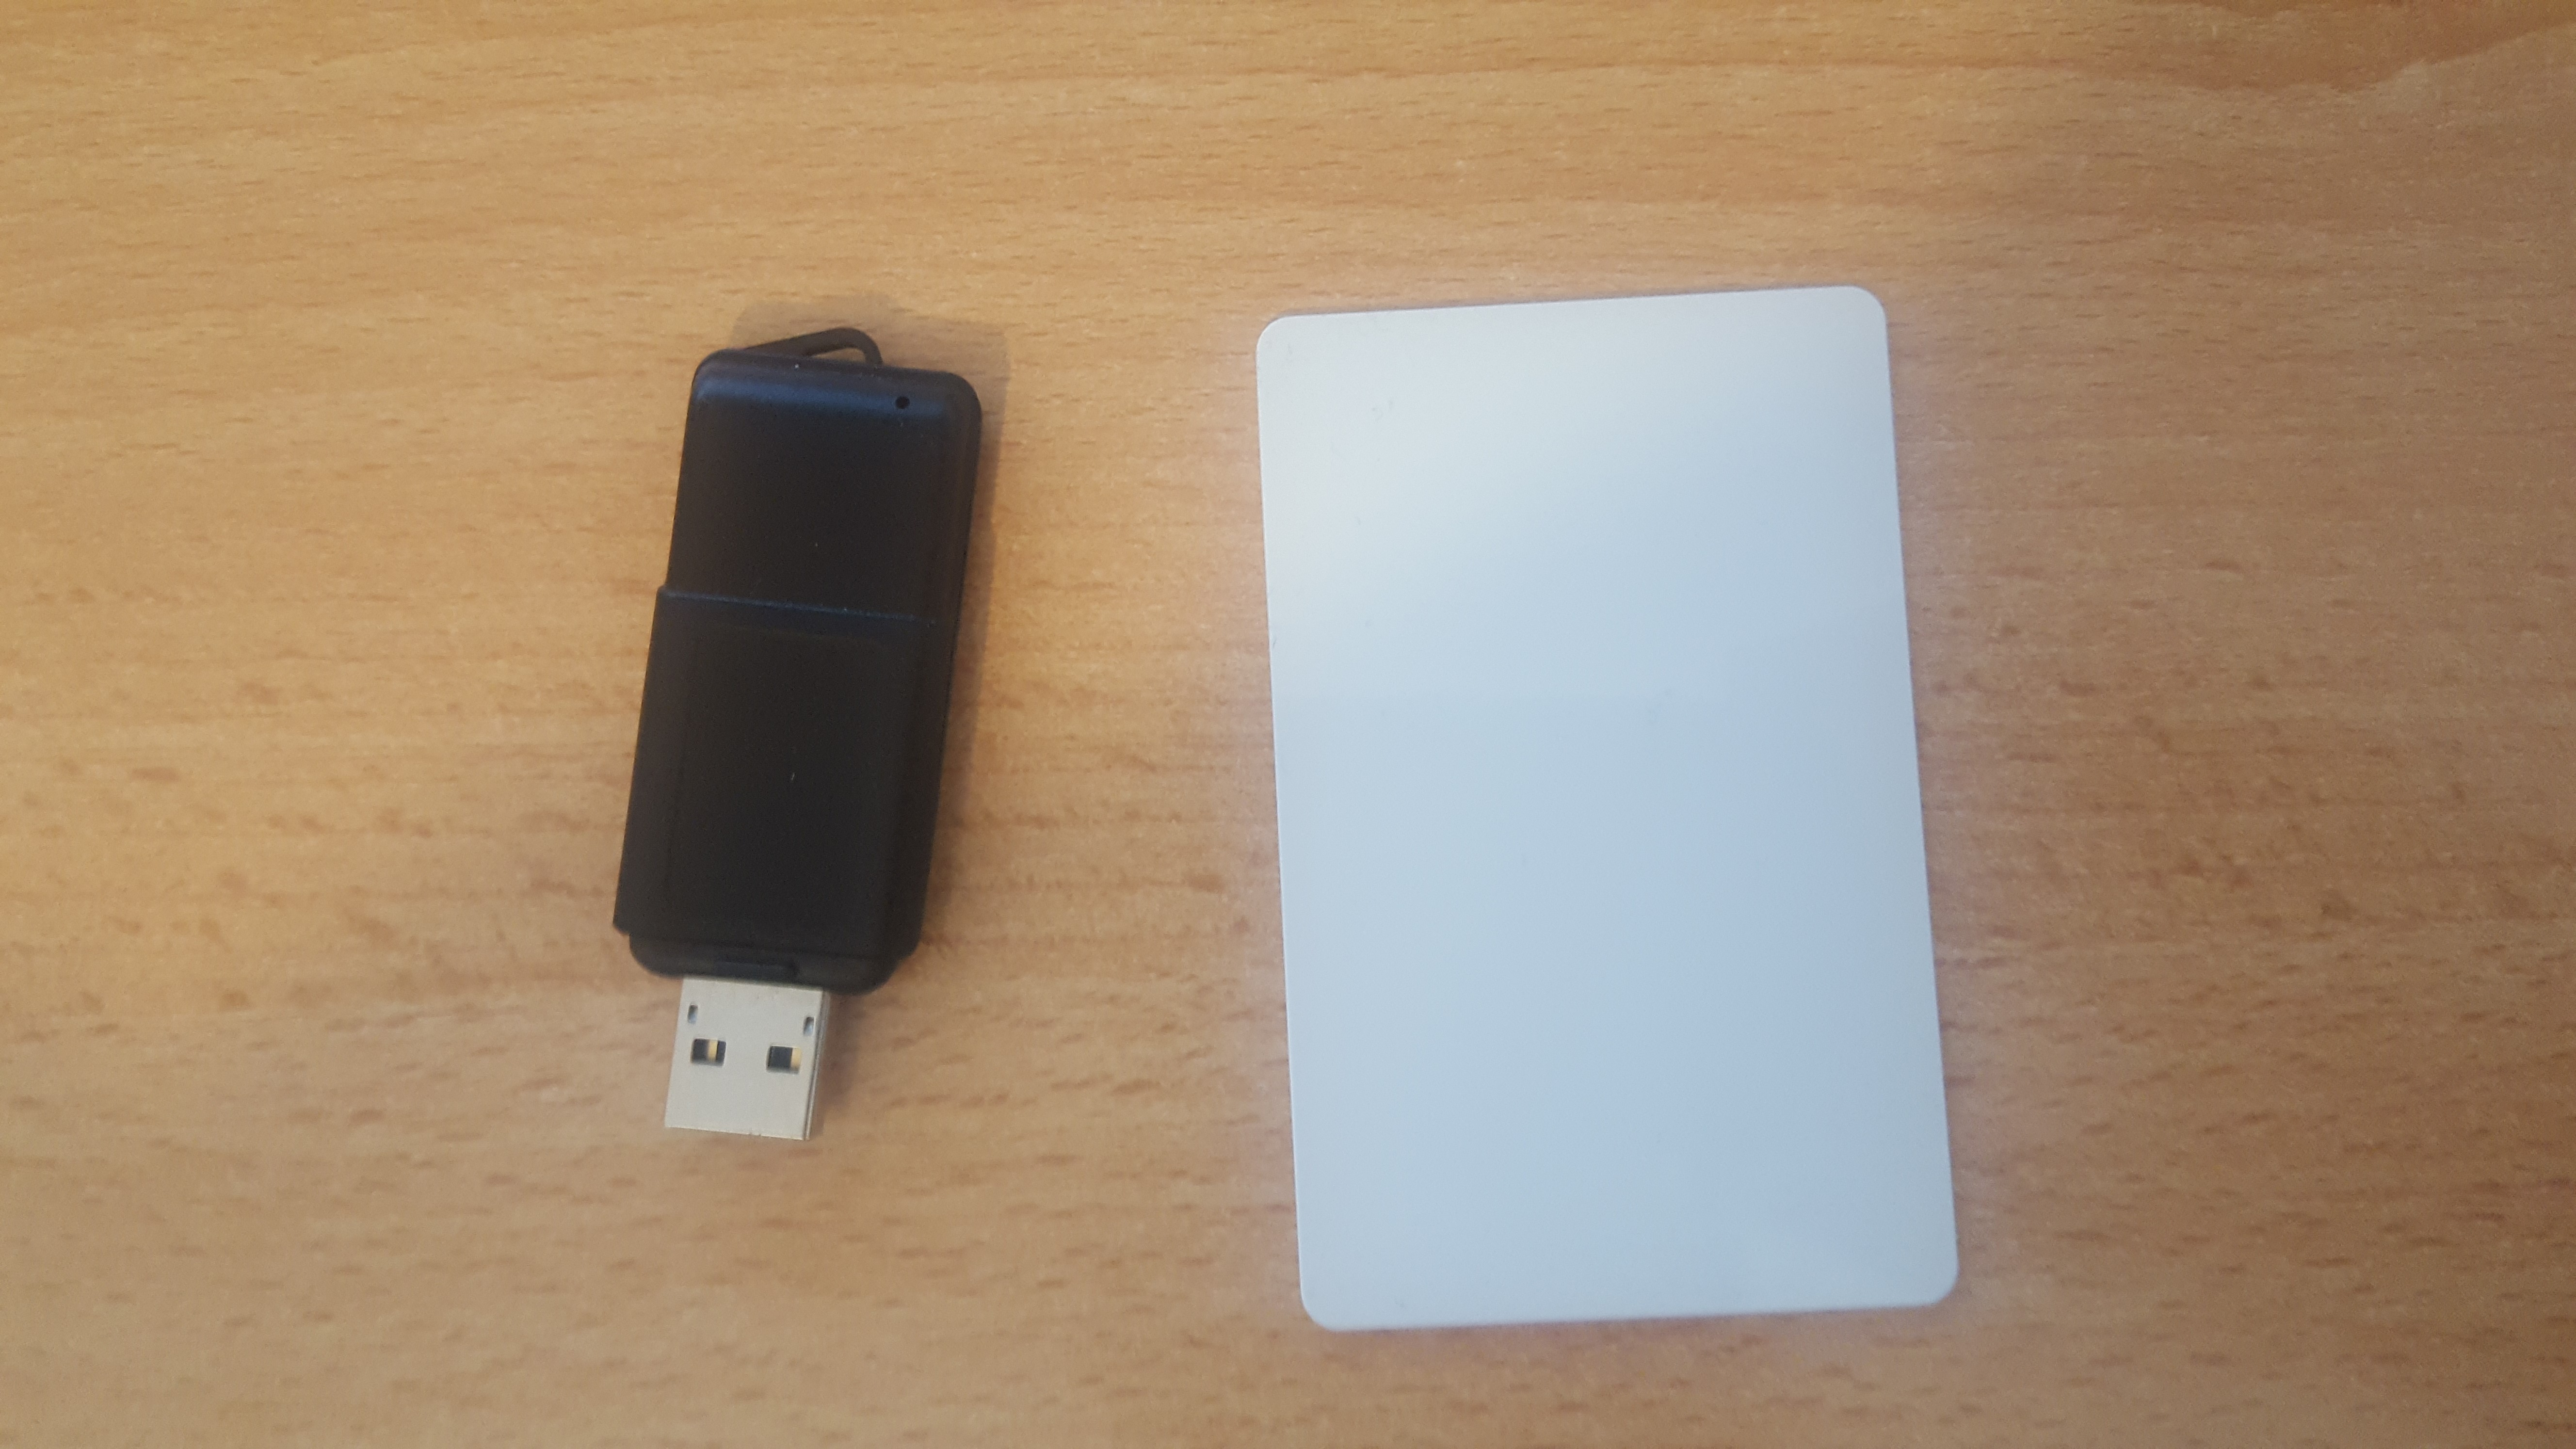
\includegraphics[scale=0.05]{introduction/hardware}

When the appropriate Smartcard reader driver is installed in an operating system, the operating system can use an appropriate library to communicate with the smartcard via the reader.


Throughout the dissertation, a number of terms are used to refer to hardware used. They will now be defined, both in terms of actual hardware used in the project, and in terms of what they would refer to in a full-scale implementation of the proposed system:

\begin{itemize}
	\item \textbf{Card:} The Java Card used, referring to either the 2.2.2 or 3.0.4 card, depending on the context.
	
	\item \textbf{Reader:} The USB Smartcard reader shown in the image above. In general, this refers to the part of the system that communicates directly with smartcards.

	\item \textbf{Host:} The Windows PC on which the authentication software runs. In a realistic implementation, this would most likely be a low-powered and cheap device and operating system, perhaps a Raspberry Pi-tye device running a lightweight Linux distribution.
	
	\item \textbf{Terminal:} This term is used throughout the dissertation to refer to the combination of host and reader.
	
\end{itemize} 

\subsubsection{Java Cards}
Java Cards are programmable smartcards which allow for the programming of applets using a defined subset of the Java language and uploading those applets to the card. They enable secure storage of data using both persistent memory as well as a small amount of RAM, and support various cryptographic functions. 

As stated on the Oracle website: "Java Card technology provides an architecture for open application development for smart cards, using the Java programming language".

Information on the development process for the Java Card platform can be found on page~\pageref{build_process}.

There are two approaches to Java Card development. “Masking” is when an applet is developed to be embedded into the card’s ROM during manufacture, alternatively an applet can be installed onto an existing card. The second method will be used for this project since it’s the easiest method for small-scale development and testing, however a for full organisation-wide rollout, masking may significantly reduce the aggregate manufacturing cost.



\subsection{Related Work}
TODO

Mention work done on Mifare and exposing weaknesses.

Any other implementation of asymmetric systems e.g. US government.

%Is this relevant? https://www2.ee.washington.edu/research/nsl/papers/ICAS-08b.pdf

%Does this have a similar result to my thing? https://link.springer.com/content/pdf/10.1007%2F978-3-642-12368-9_9.pdf

Cite paper on Opacity FS security, standards for various protocols.

Cite Denys' project from last year. Different approach, simpler more lightweight protocol.

Security Countermeasures for MIFARE Classic RFID cards - past project that summarises Mifare security.


\subsection{Project Outcome}
Overall, the project was successful, in that the success criteria have been met, and the project was completed broadly to the anticipated timetable. However, there was not sufficient time to implement any of the optional extensions suggested in the project proposal.

The primary difference between the initial project proposal and the course that the project took in reality was that in the project proposal it was suggested that there will be a full and proper comparison of available protocols. In practice, many alternative protocols were looked into briefly but it would have been difficult to  accurately assess any of them without a much lengthier investigation likely involving real implementations. There simply wasn't time.





%Preparation
\pagebreak
\section{Preparation}

\subsection{Starting point}
Prior to this project, I have had no experience with Java Cards, or smartcards in general. Most of my background knowledge in security comes from past Tripos courses, which in some cases briefly touch on material relevant to this course.

The main languages used in this project are the special Java subset used in Java Cards, and Python. Through my studies, I have gained good familiarity with Java, although the nuances of Java Card programming were previously unknown to me. I have also had a good amount of experience with Python from past work experience.

The code in the project is not developed from any pre-existing codebase but does make use of various libraries, detailed in section~\ref{subsec:libraries}, page~\ref{subsec:libraries}.


\subsection{Requirements analysis}
\label{sec:requirements}

In the project proposal, a number of success criteria were suggested. Here they are reiterated briefly discussed in terms of their context and how they might be addressed.

\begin{itemize}
	\item \textbf{The time taken for the reader to correctly authenticate the card should not exceed one second.}\\
	Smartcards have slow processing speeds, but the authentication process should be quick enough that it does not cause the user much inconvenience.
	
	\item \textbf{Access rights of a card should be revocable without having to modify the card itself.}\\
	This isn't possible with many existing systems which only rely on testing a card's knowledge of a secret key. In such systems, lost cards can continue being granted access as long as the system administrator hasn't had physical possession of the card to reprogram/destroy it. This criterion may be met by requiring cards somehow prove their unique identity, and blacklisting certain revoked cards.
	
	\item \textbf{The system should be sufficiently flexible to allow for unlimited doors, each with different access privileges.}\\
	Asymmetric cryptography will allow a system to easily meet this criterion. Each card need only maintain its own key pair, so the storage requirements won't increase with the number of encountered card readers.
	
	\item \textbf{The system should be secure}\\
	To meet this criterion, it is important to consider all probable kinds of attack. Some research into the problems with MIFARE Classic and other common vulnerabilities can inform the process, and the final system should be subjected to a security evaluation.
	
	\item \textbf{The estimated large-scale introduction cost should not exceed the typical worst-case cost of a smartcard authentication system.}\\
	This criterion should be met as long as the proposed system doesn't prescribe additional expensive equipment beyond the smartcards themselves, the authentication terminals, and a card issuing system.
	
	
\end{itemize}

\subsection{MIFARE Classic problems}
\label{sec:mifare_problems}

In December 2007, Henryk Pl\"otz and karsten Nohl gave a presentation describing the reverse-engineering of a hardware implementation of the MIFARE classic chip, and weaknesses they discovered. They published a full paper in August 2008. (TODO: links)

The pseudo-random number generator (used for key generation etc) is weak. It uses a 16b random number, blown up to 32b, to generate the initial state of a 48b Linear Feedback Shift Register. The initial random value depends on chip power-up time, so could be controlled. 

There is no nonlinear component in the LFSR feedback loop, so it can easily be reversed to find previously generated random numbers, to the system does not have forward-secrecy.

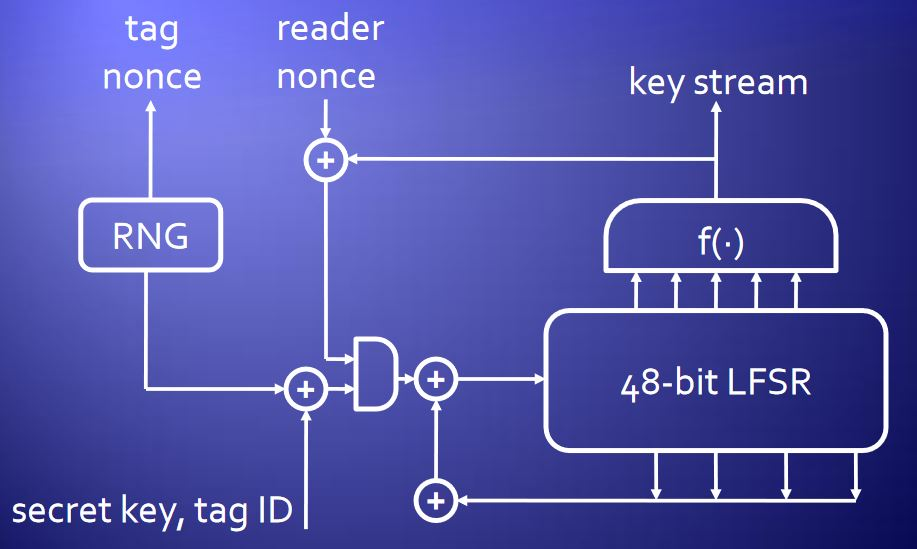
\includegraphics[scale=0.5]{introduction/mifare_classic.jpg}\\
(Figure TODO: simplified diagram of MIFARE classic key generation. (Source: presentation[TODO: LINK]) This represents the CRYPTO1 key generation algorithm, which was previously an NXP trade secret.

The actual security of the keys is far less than the implied 48b. It ultimately depends on a 16b random number, which can be brute forced easily, but even better sub-exponential attacks may exist because each key stream bit is derived from a predetermined subset of values from the LFSR which suggests non-optimal avalanche properties. %Could explain further...

As this all suggests, the security of the card was dependent on obfuscation of the implementation details, which are now known, so the card is not insecure. By controlling randomness, an attacker can even generate duplicate cards with the same initial cipher state.

While Mifare classic may still be viable for protecting low-value things such as small payments, it isn't sufficient to protect higher-value targets e.g. credit cards or access control.

\subsubsection{Attacks}
Card memory is divided into sectors, each protected by 2 cryptographic keys. The reader must supply the keys in order to access the card's memory. In a typical Mifare system, all cards protected by the same keys. Recovery of a key makes the system vulnerable. As previously mentioned, the key generation process is weak

in a research group in Radbound University Nijmegen published 4 papers about their attacks on MIFARE classic. 

Among them, "A practical attack on the MIFARE Classic" in which they extend the work of Nohl and Pl\"otz, exploiting the weakness in the pseudo-random generator to recover the CRYPTO1 keystream. They noted that nonces used to start the CRYPTO1 algorithm reappear 4 times per hour at 600,000 nonces per hour (though they can reappear in 0.618s if timing is exact) and used this to read the entire first sector, and show that they could read any sector provided that they know the content of one memory block in that sector.

Another of the papers is "Wirelessly pickpocketing a MIFARE classic card" in which they outlined 4 attacks that only require a wireless reader, which are briefly summarised below:
\begin{enumerate}
	\item Mifare parity bits computed over plaintext, not cipher text, so they leak information. Only about 1500 authentication attempts necessary, then 48b offline brute-force attack to break the cipher.
	
	\item Also exploits parity bit weakness. Adaptive Chosen Ciphertext Attack with about 28500 adaptively chosen challenges to the card. Guarantees only 436 possibilities for odd-numbered bits of the internal cipher state. This reduces the offline search space to 33b.
	
	\item Attacker keeps challenge to the card constant, varying the challenge from the card to the reader until a special internal cipher state is reached. Special states are precomputed and placed in a 384GB table. Requires around 4096 authentication attempts, with a few extra for more efficient table lookup.
	
	\item Assume attacker has already recovered one sector key. Authenticate for that sector and then a new sector. Challenge nonce for new sector is encrypted with new sector key. Because of the 16b random number generator and that parity bits leak information, the attacker can easily calculate the plaintext nonce and hence 32b of the keystream. Use this to generate around $2^{16}$ candidate keys. Requires 3 authentication attempts and under a second offline search.
\end{enumerate}

Numerous other attacks have been used that are variations on the above. In April 2009, a better Conditional Multiple Differential card-only attack was found, first announced by Nicolas T. Courtois at Eurocrypt 2009.

\subsubsection{Problems with successors}
Some brief comments on security vulnerabilities of successor systems:

In 2011, NXP replaced Mifare classic with the backwards compatible Mifare Classic EV1, which was resistant to the card-only attacks known at the time. However, a new card-only attack for the EV1 was found in 2015.

Mifare DESFire cards were shown to be insecure in 2010 when it was shown they could be cloned for about \$25 in easily available hardware. Other problems were also discovered.

Mifare Ultralight is also vulnerable to some attacks.

\subsection{Preparation strategy outline}
The development approach decided on for this project was the Waterfall model, because it fits the project much better then alternatives such as a spiral model or evolutionary model. This is because it is a relatively small project, completed by one person, within a limited time and with known requirements. It is most likely that, once some basic decisions have been made such as which protocol to implement, the first working prototype will be very close to the final project.

Waterfall model steps:
\begin{itemize}
	\item \textbf{Requirements:} Already set out in the project proposal. TODO: Should I include it and reference it?
	
	\item \textbf{Specification:} The process of refining the requirements to a more detailed specification is done in multiple parts. It is first touched upon in the requirements analysis section (page~\pageref{sec:requirements}), and further considered throughout the project when important decisions are made, such as the choice of protocol or authorisation method. %Could reference these sections
	
	\item \textbf{Implementation \& unit testing:} Implementation details are discussed throughout the Implementation section, with unit testing occurring throughout as described in the upcoming subsection, \ref{subsec:testing}.
	
	\item \textbf{Integration \& system testing:} All the individual components were used together without special code for testing individual functions. The nature of the task limited the amount of modularity available beyond the distinction between card and host code, so integration wasn't a big task. Testing consists of running the system as a whole using automatically generated values and some fixed test parameters.
\end{itemize}

It should be noted that the system is security-critical. This should be reflected in my implementation and testing strategy. For instance, the chance of data being stolen from any part of the system during online operation that may compromise the system has to be considered, and all possible points of weakness have to be considered. The system's security properties are assessed in the Security Analysis section, page~\pageref{sec:security_analysis}.

\subsubsection{Project structure}
The project will be split into modules that logically follow from the inherent divisions in the work. Card issuing and card authentication will be implemented separately, key algorithms will be separated into their own functions rather than integrated into large sections of code, and so on. 

Ease of modification is also a consideration. For instance, constants often occur multiple times in protocol implementations, so all the important constants are separated out into a separate class file.

\subsubsection{Testing}
\label{subsec:testing}

Testing and debugging can be performed on the host-side component of the system relatively easily, as with any other body of code.

Testing and subsequent debugging on the Java Card component is much more difficult, since unlike in a conventional program, a developer doesn't have the option to easily see program data during runtime and ensure they match expected values. The nature of the hardware means that each APDU command to the card can only result in a single response APDU, containing a limited amount of data and a response code. As a result, testing and debugging could only be done as a series of separate executions, using breakpoints at various stages in the code and returning the relevant data, thus terminating the program. There is certainly no way to, for instance, step through the code line-by-line and follow the execution process to identify exactly when a problem occurs. %Could mention simulations.

% TODO: describe system test.

% TODO: Get code snippet of this.


\subsection{Safety case}
TODO: format this nicely.

(outline hazards and risks, strategies for dealing with them\\
Possible hazards and risks:

Card lost/stolen. Owner reports it missing, a good system would allow the administrator to revoke cards without needing physical access to the card.

Card wrongly issued. Once the mistake is detected, the card would have to be blacklisted from all terminals using it.

Card issued with wrong permissions. This would be due to either human error on the part of the issuer, or deception on the part of an attacker. Measures taken would depend on the exact system implementation, but may involve blacklisting the card at certain terminals the card was mistakenly granted access to, but this can only be done after the mistake is identified. A good way to mitigate the risk of this is to have clearly defined, unambiguous "permission profiles" for the issuer to choose between e.g. student, researcher, etc.

Keys are stolen by the attacker directly. This would mean that a card could spoof copies of the card which was assigned that key. The main problem is detecting that an attack has happened, as it may be possible to steal a key without the owner knowing. Terminals should keep a log of cards that access it, and any suspicious use of cards with that key will cause the system administrator to check the log and blacklist that particular key. The legitimate owner would then be forced to obtain a new card.

Some master key used to sign certificates is compromised. Very bad for the system since it means that any attacker can forge their own valid certificates. For this reason, keep this key separate from the wider network. Good solution is to have a card generate \& store it, and generate valid certificates. This way, nobody can know what the key actually is, and the security measures of the card makes it virtually impossible to steal the key even if an attacker has access to it.


\subsection{ISO7816}
Throughout the dissertation, I will reference certain things defined by the ISO7816 smartcard standards. Here is an overview of the main ones.

\subsubsection{Application Identifiers}
\label{subsec:aid}
TODO

Explain AIDs. Structure specified in ISO7816.

Resource Identifier 5B long, Proprietary Identifier Extension PIX 0-11B long.

\subsubsection{APDUs}
An APDU, or Application Protocol Data unit, is the data format used in communication between the card reader and the smartcard. Communication occurs in command-response pairs in which the reader initiates an exchange with a "command" APDU, and the card responds. The formats of these APDUs are defined in ISO7816-4.

APDUs facilitate stateless network-layer communication, analogous to HTTP, which results in a client-server model in which the card acts as the server. Any continuity between consecutive interactions between the reader and card must be implemented at a higher level, for example by including IDs in the data section of APDUs.

The following table is taken from the ISO7816-4 part 5.1. It shows the actual structure of the APDU command-response pairs

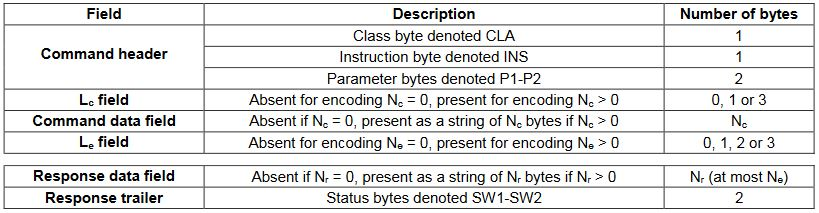
\includegraphics[scale=0.7]{introduction/apdus}

Brief summary of the fields:

\begin{itemize}
	\item  Class byte - type of command. bit 8 $b_8=0$ means interindustry class and the format is quite restricted. $b_8=1$ means proprietary class.
	
	\item Instruction byte - indicates the specific command.
	
	\item Parameter bytes - parameters for the instruction. In some cases, more convenient than using the data bytes.
	
	\item $L_c$ specifies how many bytes follow in the data field
	
	\item $L_e$ specifies the maximum number of data bytes that the smartcard is permitted to return to the reader.
	
	\item Command/Response Data field - Arbitrary application-defined data.
	
	\item Status bytes - Values returned to indicate whether the instruction was successful, or what error occurred. 0x9000 indicates that the instruction was executed by the card successfully. (TODO: explain other status words)
\end{itemize}


%TODO: Cover SELECT, other special APDU types



\subsection{Development Preparation}
Before work can begin on the main implementation, I need to invest time in ensuring that I fully understand the steps involved in the development process, that everything is set up correctly and that appropriate decisions are made regarding the structure of the project.

I decided that the text editor Atom would be used to write the code, since it can easily be configured with IDE plugins for multiple languages simultaneously, allowing for both the host-side and card-side application to be developed side-by-side.

Additionally, I ensured that the project file structure was reasonable and configured the relevant environment variables to facilitate the use of the development tools.


\subsubsection{Version control}
One of the first steps taken in preparation for beginning the development process was to ensure that there was a good system for remote backup and version control in place, in case work was lost or corrupted locally, or big mistakes were made and it became necessary to roll back the code to a previous version. I used GitHub for this, ensuring that everything of value was included in the backup, not just the code itself, but also all notes, scripts and documentation.

\subsubsection{Java Card 2.2.2 Build process}
\label{build_process}

Initially, development took place using the Java Card 2.2.2 platform, and the following describes the process of developing applets for this version.

Setting up the development environment involved fixing a project structure and configuring environment variables, such as setting JC\_HOME to the Java Card library files, setting PATH to allow Java Card development tools to be used from different directories, installing the relevant library files, and ensuring the Java classpath contains the API and installer .jar files.

\textbf{Compiling:} As with many other types of project, the first step is compiling the code. The compilation of Java Card code uses the standard "Javac" Java compiler, and only requires that the api.jar and installer.jar libraries are included in the classpath. The api.jar library enables the use of Java Card library functionality and the installer.jar library allows the build to be installed onto the card. The source and output should be a version compatible with the Java Card version used. The \verb|-g| option to generate all debugging information is required for the converter step.
\begin{verbatim}
-javac -g -source 1.5 -target 1.5 -cp ".\bin;
    ..\..\..\java_card_jdk\2.2.2\java_card_kit-2_2_2\lib\api.jar;
    ..\..\..\java_card_jdk\2.2.2\java_card_kit-2_2_2\lib\installer.jar" 
    -d .\bin src/uk/ac/cam/bo271/applets/opacity_zkm/*.java 
\end{verbatim}
The output is in the form of .class files.

\textbf{Converting:} This step is required to convert the class files to a format compatible with Java Cards. This step checks for any programming practices incompatible with the Java Card platform, such as the use of the 'int' data type, or structural errors such as the lack of an applet class. The format for the command is as follows:
\begin{verbatim}
converter [options] <package_name> <package_aid> <major_version>.<minor_version>
\end{verbatim}

The Package name is the name of the package to be converted into an applet, such as "uk.ac.cam.bo271.applets.helloworld". An AID, or Application Identifier, is a value allowing an applet to be uniquely identified (more details in section~\ref{subsec:aid}, page~\pageref{subsec:aid}). The Package AID is the AID of the entire package, not of a specific applet. Without specifying an applet AID, the package can only be used as a library by other applets. Specify an applet using the option 
\verb|-applet <AID> <class_name>|, where AID must have the package AID as its prefix.

\begin{verbatim}
-call converter -exportpath 
     "..\..\..\java_card_jdk\2.2.2\java_card_kit-2_2_2\api_export_files;
     .\JCMathLib\bin" -classdir .\bin 
     -applet 0xD1:0xD2:0xD3:0xD4:0xD5:0xD6:0x01
     uk.ac.cam.bo271.applets.opacity_zkm.Opacity 
     uk.ac.cam.bo271.applets.opacity_zkm 0xD1:0xD2:0xD3:0xD4:0xD5:0xD6 1.0
\end{verbatim}

The output is a file in the form of a CAP (Converted APplet) file, with the .cap extension, e.g. \verb|helloworld.cap|, which can then be uploaded onto the card. 

\subsubsection{Differences in Java Card 3.0.4 Build Process}
The installation process had to be revised midway through the project. This was due to the migration from java card 2.2.2 to 3.0.4 (section~\ref{subsec:version_change}, page~\pageref{subsec:version_change}). The new process was different and had virtually no documentation, but I found an Apache ANT task which performs the compiling and converting stages. First a 'build' file had to be produced in XML format, specifying the Java Card development kit path, the ANT task, AID, package etc. and making a call similar to:

\verb|ant -buildfile ant_tasks\build_opacity_opt.xml|

TODO: Stick example build file in appendix.

\subsubsection{Uploading and running applets}
For both the versions described above, the upload process is almost identical. Once the applet is converted to a CAP file, it can be uploaded into the card using a GPShell script.

GPShell is a scripting tool that implements the GlobalPlatform specifications, which determine the management of applets on a smartcard. It generates a series of APDU commands conforming to the GlobalPlatform specifications which upload the applet to the card.

In the following example GPShell script, the connection to the card via the reader is established, and the security domain applet is selected. This is what performs the applet management. For the GP211 specification, some card manufacturers set this as A000000151000000, others use A000000003000000.

A secure channel is then opened, any existing version of the applet deleted, and the .cap file is installed, and the connection is terminated.
\begin{verbatim}
mode_211
establish_context
card_connect
select -AID a000000151000000
#select -AID a000000003000000
open_sc -security 1 -keyind 0 -keyver 0 -mac_key 404142434445464748494a4b4c4d4e4f 
        -enc_key 404142434445464748494a4b4c4d4e4f
delete -AID C1C2C3C4C5C601
delete -AID C1C2C3C4C5C6
#install -file ..\code\applets\bin\uk\ac\cam\bo271\applets\challengeresponse
               \javacard\challengeresponse.cap -sdAID a000000003000000 -priv 2
install -file ..\code\applets\bin\uk\ac\cam\bo271\applets\challengeresponse
              \javacard\challengeresponse.cap -sdAID a000000151000000 -priv 2
card_disconnect
release_context
\end{verbatim}

A full APDU trace for the upload script is available in TODO: appendix (also explain what APDUs do in the appendix section).

Other tools exist for uploading .cap files, such as the 'apdutool' program supplied in the Java Card development kit, but I found GPShell was more flexible and usable.

\subsubsection{Practice}
Before starting work, I had to gain familiarity with the aforementioned tools and processes, and find the best approach.

First, used GPShell and a pre-compiled test applet in .cap format that came with it to write a test script to upload the applet, list contents, and  uninstall it.

Then I attempted to run an applet using host-side code. Initially I attempted to use OpenCard Framework, and when that didn't work I switched to an appropriate Python library (section~\ref{subsec:python_pcsc}, page~\pageref{subsec:python_pcsc}), which worked for the simple "hello world" applet.

The Java Card development kit comes with some source code for sample applets that demonstrate applet structure. I used these to test the compilation and conversion steps, and then uploaded a simple one to the card to ensure everything worked properly. I had some initial problems due to using the incorrect JCDK version which was incompatible with the cards, but it worked eventually.

The next step was to write a simple command-response test applet that stored an input string, and returned it later. In this step, I learned about the various quirks and limitations the Java Card library and platform (e.g. int-to-short casting, restrictions on APDU passing, different garbage collection system). This took quite some time as online resources for Java Card development is scarce.

At that point I judged that I had learned the development procedure well enough to begin development of the main applet. It was then easy to combine all the main steps; compiling, converting, uploading and running, into shell scripts that allow new builds to be executed with minimal effort. An example script for the Java Card 3.0.4 build is as follows:
\begin{verbatim}
call ant -buildfile ant_tasks\build_cr.xml
GPShell.exe gpshellscripts\crinstall.txt
python ..\code\Python\Challengeresponsehost\ChallengeResponse.py
\end{verbatim}

\subsection{Host to Card interface}
To develop applications that run on some conventional Windows/Linux operating system which can communicate with a contactless smart card, a suitable card reader is required, as well as suitable libraries that provide access to the functionality of the reader.

\subsubsection{OpenCard Framework}
Initially, the OpenCard Framework was identified as a potential Java-based middleware/API that could be used for developing the host-side part of the project. It was developed many years by the OpenCard Consortium and mostly driven by IBM (TODO: reference website).

However, upon writing some code for a sample project and attempting unsuccessfully to run it, I noted that the framework was failing to recognise the card reader.

after much frustration, I discovered that the OpenCard framework must be explicitly implemented by the smartcard reader for the middleware to work. Many commercially available readers, including  the one used in this project, do not support it, and instead only support the more common PC/SC framework. My initial assumption had been that OpenCard was a wrapper for PC/SC, but this was disproven by the fact that some reader data sheets specify PC/SC and OpenCard whereas others only specify PC/SC.
%Could back up claim that only some cards support OCF

\subsubsection{PCSC}
After the failed attempt at using the OpenCard framework, it was clear that PC/SC was required. 

PC/SC is a standard API that interfaces smartcards and smartcard readers with a PC. Windows comes with a PC/SC implementation by default, while there exists a less complete but perfectly functional implementation for Linux and Mac OSX, called PC/SC-lite. 

The PC/SC API is implemented in C, though various bridges/wrappers exist for other languages. Not all languages have a library for PC/SC support, but many do, including Java, Visual Basic, and Python.

\subsubsection{Python PC/SC wrapper}
\label{subsec:python_pcsc}

%Could stick this in implementation chapter

Not all common languages have good library interfaces with the PC/SC API, but many do. The choice of language for the host-side implementation was motivated far more by language preference than by necessity.

Python has the library 'pyscard' (PYthon Smart CARD), developed by Gemalto, which interfaces with both PC/SC on Windows and PC/SC Lite for Linux/OSX. The Python language is itself highly portable, and the portability of the library meant that I could develop on Windows in the knowledge that it could be easily ported to a low-power Linux system that could act as a real-world door controller. This motivated the choice of Python.

Another motivation for choosing Python was that the nature of the language suited the kind of development that would be undertaken. At the beginning of the project, I had no experience with smartcard development and knew that I would constantly be testing various things and changing code rapidly. The Python language makes quick modifications and tests very easy. Further, I had lots of experience with Python prior to beginning this project, so it was convenient to not have to learn a new language.

Upon testing, the pyscard library worked well.

TODO: include code snippet



%Implementation
\pagebreak
\section{Implementation}
%Could add more things in here relating to learning dev process.

\subsection{Chosen Protocol - opacity ZKM}
TODO: Reference the other protocols looked at, mention that they were briefly examined and Opacity ZKM seemed to fit the requirements best.

The Opacity protocol standard defines two protocols; Opacity ZKM (Zero key Management) and Opacity FS (Full Secrecy). The main difference between the two is in the authentication of the terminal. Opacity ZKM doesn't require the terminal contain any secrets and therefore cannot be authenticated by the card, whereas Opacity FS requires terminals have certificates much like cards, which can be authenticated by the card.

\subsubsection{Brief overview}
This is a high-level description of what the Opacity ZKM protocol does in order to authenticate a card.
\begin{itemize}
	\item Cards issued with certificates signed by root key
	\item Both sides perform ECDH, use the result to derive session key
	\item Use session key to generate a Message Authentication Code using CMAC for session-specific data, proving the card knows the private key corresponding to its certificate.
	\item Card sends the nonce, MAC, and certificate to the terminal
	\item Terminal uses the root public key to verify the certificate, and checks the MAC value.
\end{itemize}

%Describe auxiliary protocols
\subsubsection{EC Crypto}
TODO

brief description of EC Cryptography

Elliptic Curve Cryptography is a form of asymmetric (public-key) cryptography. 

Talk about operators */+

The Opacity protocol uses elliptic curve cryptography, in two areas.
\begin{enumerate}
	\item Authentication: The Elliptic Curve Diffie-Hellman algorithm is used to establish a shared secret between the two ends over a potentially compromised channel. See the next section for further details.
	
	\item Certificate signing: The Elliptic Curve Digital Signature (ECDSA) algorithm is used by a central card issuing service to provide unforgeable proofs of authenticity of card certificates.
\end{enumerate}


\subsubsection{ECDH}
\label{subsec:diffie_hellman}

\textbf{Key exchange }(or key establishment) is any process by which cryptographic keys are exchanged between two parties to enable cryptographic methods, particularly encryption/decryption, to be used in communication between the parties. In general, key exchange may either be done via the same channel that will be used for  encrypted communication (in-band key exchange), or using a separate channel (out-of-band key exchange). 

The \textbf{Diffie-Hellman Key Exchange} is one of the earliest asymmetric cryptographic protocols, using asymmetric cryptography to negotiate a shared secret value across an insecure medium such that both parties will end up sharing a secret which no eavesdropper can reproduce.

In the most general case, there is some agreed cyclic group $\mathbb{G}$ and a generator $g$ for the group $g$. These can be public. 

A has a secret key $x \in \mathbb{G}$, B has a secret key $y \in \mathbb{G}$. A computes $g^x$ and sends to B, and B computes $g^y$ and sends to A. A and B can then take the received value to the power of their own secret key, calculating $g^{xy}=g^{yx}$. This value is the shared secret.

Secrecy is ensured due to the \textbf{Discrete Logarithm Problem}, which states that it is computationally infeasible for anyone with access to any $g^s$ to calculate $s$ (and in fact, there may be many solutions to the discrete logarithm, only one of which is the original power). An eavesdropper also cannot calculate the shared secret $g^{xy}$ from knowledge of $g^x$ and $g^y$ for this reason.

The \textbf{Elliptic-Curve Diffie Hellman} protocol is one kind of implementation of the Diffie-Hellman key exchange method, done with Elliptic Curve cryptography.

In the Opacity ZKM protocol, the EC-DH step is one of the first actions performed by the card and terminal. It uses the card's persistent keypair and the host's ephemeral keypair to establish a shared secret which is the basis for further steps. It is necessary to assume the channel is compromised due to the use of wireless communication, which can easily be intercepted by an eavesdropper, making the use of EC-DH a logical approach.


\subsubsection{ECDSA}
ECDSA, or Elliptic Curve Digital Signature Algorithm, is a version of the Digital Signature Algorithm (DSA) using Elliptic Curve cryptography.

A Digital Signature is a construct in public-key cryptography for proving the authenticity of the source of some information. The owner of a key pair "signs" some information using their private key, and any other party can verify that the signature was produced by the keypair owner using the corresponding public key. 

%Could explain further how ECDSA works if more content needed.

The purpose of its use in the Opacity ZKM protocol is to verify the authenticity of the CVC certificates issued to the terminal by the key issuing authority. During the authentication process, the terminal uses the issuing authority's public key(s) to verify that the certificate is genuine, proving that the public key used by the card and included in the certificate corresponds is one that was validated by the certificate issuing authority.

\subsubsection{ASN1}
ASN.1, or Abstract Syntax Notation 1, is a standard for data encoding. There are multiple ways it can be used, and the ASN.1 format used in Opacity is the BER (Basic Encoding Rules) format, which is primarily used for formatting and parsing the certificate. 

Values are encoded in "TLV" form (Type-Length-Value). Complex data formats can be achieved by combining primitive and constructed data types, for example using the "sequence" type which consists of a sequence of other TLV values.

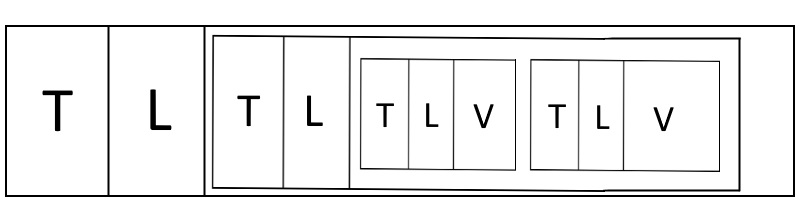
\includegraphics[scale=0.5]{implementation/tlv}

During the card issuing stage, a new certificate has to be created. It makes far more sense for this to be done by the issuing host device, rather than the card, since it can be done much faster and the host must generate the signature for the certificate in any case.

\subsubsection{CMAC}
\label{subsec:cmac}

A MAC, or Message Authentication Code, is a code that proves that a message was sent by the claimed sender, and was not modified in any way. It uses symmetric cryptography, so a MAC generated for a particular message by one party using a shared secret key can only be verified by another party also sharing this key, typically by also calculating the MAC of the message with that key and verifying it matches the received MAC.


(TODO: credit images found on wikipedia)\\
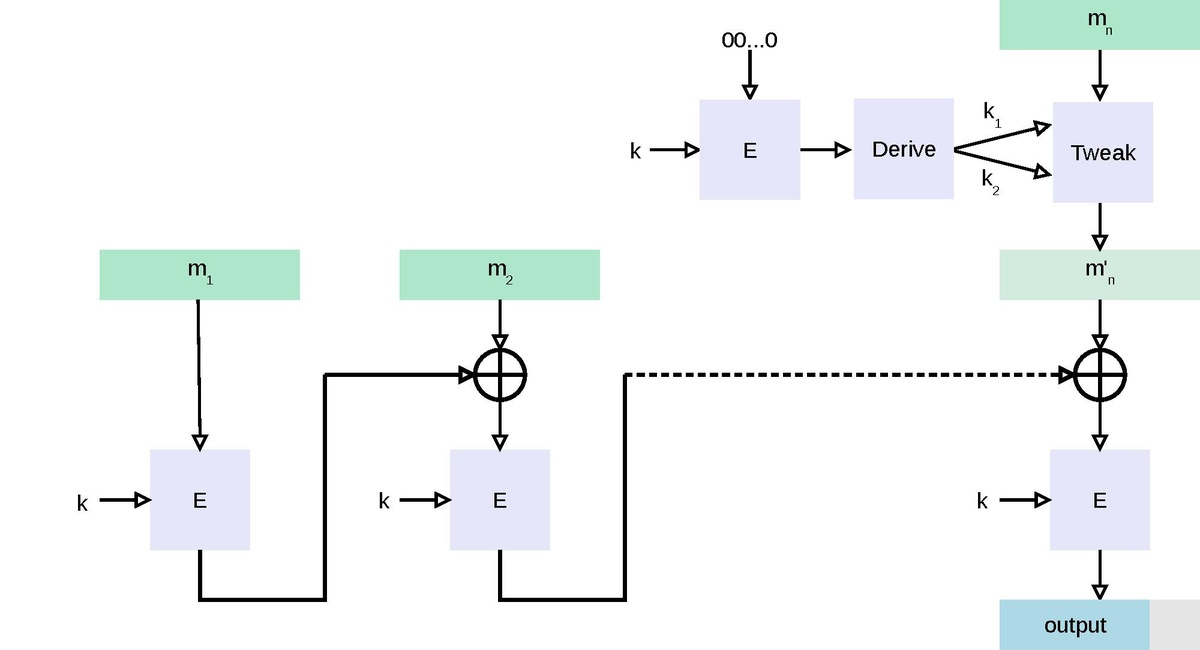
\includegraphics[scale=0.5]{implementation/CMAC}

Defined in NIST 800-38B

The best way to describe the C-MAC algorithm is to describe it as an extension of the CBC-MAC algorithm, which uses the CBC (Cipher Block Chaining) block cipher mode of operation. The link between the two can be easily seen by comparing the CMAC diagram with the following diagram outlining CBC-MAC:\\
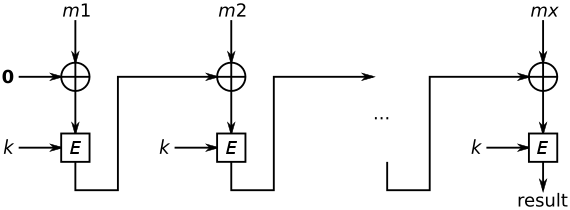
\includegraphics[scale=0.5]{implementation/CBC-MAC}\\
Of course, $\mathbf{0} \oplus m1=m1$ so the initial step is identical to C-MAC. The difference is in the treatment of the final block of the message. In the CBC-MAC case, the final block is treated the same way all all the others, with the final cipherblock being used as the MAC.

(TODO: wiki reference, this part is mostly copied from CBC-MAC Wikipedia page)\\
This is secure for messages of an agreed fixed length, but not for variable-length messages.

If two correct message-MAC pairs $(m,t)$ and $(m',t')$ are known, an attacker can generate a third message $m''$ with the MAC $t'$ as follows: 
$$m''=m||[[m'_1\oplus t] || m'_2 || \cdots \\ || m'_n]$$
This is because upon computation of $\text{MAC}(t)$, the MAC $t$ produced after $m$ has been processed will be XORed with $[m'_1 \oplus t]$, giving $m'_1$, and the rest of $m_1$ will be processed identically to if $m_1$ were processed by itself. C-MAC fixes this problem by XORing the final block $m_n$ with one of two subkeys derived from the primary key $k$ before executing CBC-MAC, which can't be replicated by the attacker who can't account for this step.

In the Opacity ZKM protocol, the input length for C-MAC is in fact fixed at 38B so the use of C-MAC rather than something like CBC-MAC isn't strictly necessary, but has no disadvantages (Other than that it was not supported by the Java Card versions used, see page~\pageref{cmac_impl} for implementation details).

The purpose of the C-MAC step in the Opacity ZKM protocol is to generate a 

Incorporates host and card IDs, and ephemeral host public key, so the input is different every time. Because the host's public key is ephemeral, the C-MAC value is different each time, so the card proves by executing the C-MAC on this information that it derived the correct session key $\text{SK}_{\text{CFRM}}$. This implies that the card completed the key derivation step successfully, which in turn implies that the card shares the secret with the host, either through an EC-DH step, or from a previous interaction (Persistent Binding optimisation, section~\ref{subsec:pb}, page~\pageref{subsec:pb}), proving that the card knows the private key corresponding to the public key in the certificate it claims ownership of. 

%Could describe why MAC is preferable to a signature. Easier to compute?



\subsubsection{Key derivation}
\label{subsec:kdf}

The key derivation function is used to derive a set of session keys, as well as next time's shared secret if the persistent binding optimisation is used, from this session's Elliptic Curve-Diffie Hellman shared secret (or from the previous interaction's derived key values if the optimisation is used).

The function used in the protocol is defined in the NIST SP 800-56A standard, section 5.8.1. It involves creating an arbitrarily long sequence of pseudo-random bytes by repeatedly taking the hash of an incrementing counter value with shared secret $Z$ and some session-specific 'info' data including random data from both parties to ensure that the only way to calculate the key data is by knowing $Z$ (and not saving previous key data and fixing this interaction using the same parameters, for instance). 
\begin{align*}
\text{DerivedKeyMaterial} =\ &\text{hash}(0\text{x}00000001||Z||\text{info})||\\
&\text{hash}(0\text{x}00000002||Z||\text{info})|| \cdots\\
&\text{hash}(0\text{x}00000000+n||Z||\text{info})\\
\end{align*}


%outline program structure with code snippets
\subsection{Java Card Protocol Implementation}
%First: outline basic features of javacard application. (could be moved to preparation section)

%Give good code abstractions, explain overall design decisions. 

This section describes the base implementation. For details about optimisations, see section~\ref{sec:optimisations}, page~\pageref{sec:optimisations}.

\subsubsection{Program structure}
%Could Move to Preparation Java Card section depending on word counts.

All Java Card applets must adhere to a basic program structure, which is modelled by extending the abstract "Applet" class and implementing the methods included in it. Only classes extending the Applet Java Card library class can be directly interacted with when uploaded onto the card, though other classes may be included in the package and used by the applet class. The primary methods that should be implemented are \verb|install()|, and \verb|process(APDU apdu)|, though other methods may optionally also be implemented.

The static \verb|install()| method called when applet is first installed. It should create a new instance of the applet class, in my case by executing \verb|Opacity applet = new Opacity();|. It should then call the \verb|register()| method on the new applet instance (TODO: why?). Either the \verb|install()| method, or the applet's constructor, should initialise the state of the applet and create persistent objects in EEPROM which are to be used in later interaction.

The \verb|process(APDU apdu)| method is the point of entry into the applet for typical runtime use, executed when that applet is currently selected and a new APDU is received from the terminal, where the APDU is encoded into a Java Card "APDU" object and given as the argument. The \verb|process()| method takes an appropriate course of information based on the information contained within the APDU. My implementation ensures the class code is 0x80 (user-defined), and executes a switch-case statement on the instruction code. A subsidiary function is then called depending on the instruction code. This allows modularity at the level of high-level functions, and easy modification of supported functionality.

TODO: include code snippets. 

%Could discuss limitations in how APDU is passed, lack of int type, standard libraries inaccessible, different libraries exist etc

%\subsubsection{Memory management}
%Outline different types of memory, how they're allocated.

%Mention what things should be persistent or transient. Absolutely necessary that recurring things should be persistent. Reference parts of Opacity protocol that require this e.g. certificate, key pair. Persistent ID prevents recomputation etc.

\subsubsection{CMAC}
\label{cmac_impl}

CMAC was not implemented in either Java Card version I attempted to use (2.2.2 or 3.0.4). It was only introduced in 3.0.5 (reference cards not yet available). Consequently, I had to implement it myself. 

I deemed it best to write an implementation that can be used in virtually the exact same way as if it were a library implemetation, so I wrote a class AESCMAC128 which extends Signature (the abstract class for digital signatures). The instance would be created in the Opacity class constructor and stored in EEPROM. It would make use of transient byte arrays because operations would not need to be performed across multiple accesses.

On the Java Card 2.2.2 platform, I used the \verb|ALG_AES_MAC_128_NOPAD| mode of the Signature class as an auxiliary function in the C-MAC algorithm. For unknown reasons, this option didn't work in the version 3.0.4 cards I had acquired, so instead I made use of the structural similarity to CBC-MAC, using the AES-CBC mode of the Cipher class. Both of these approaches worked well.

%TODO: Maybe more in-depth implementation details.

See section~\ref{subsec:cmac}, page~\pageref{subsec:cmac} for a general description of the C-MAC algorithm.

\subsubsection{ECDH}
With the Java Card 2.2.2 version, the library implementation of ECDH proved to be a big problem. Ordinarily, the shared secret outputted by ECDH using 256b elliptic curves would be the 32B result of the point-multiplication operation with one party's private key and the other party's public key. However, in the Java Card 2.2.2 implementation, it only returned the 20B SHA-1 hash of this value.

This was useless in implementing the Opacity protocol, since the shared secret is required in its raw form as an input to the key derivation function (section~\ref{subsec:kdf}, page~\pageref{subsec:kdf}).

Initially an attempt was made to implement elliptic-curve point multiplication manually, though as described in section~\ref{subsec:version_change}, this attempt failed, forcing the move to the Java Card 3.0.4 platform, which supported returning the raw ECDH value rather than the hash.

\subsection{Host-side implementation}
As described in (TODO: reference), the host application was done using Python, with the Pyscard library for interfacing with the USB card reader and communicating with the card. In this section I will give some some details about how it was implemented.

Using this library, the Python code was able to successfully communicate with the card. Some information required for the process to success, such as the root key required for certificate authentication, was stored as separate files in the same directory as the code. A full system implementation would likely use a different structure but the principle is the same, so it makes sense as an approach to prototyping the system.

As with the previous section, this only deals with the core implementation. Details pertaining to protocol optimisations such as the Persistent Binding optimisation can be found in (section~\ref{sec:optimisations}, page~\pageref{sec:optimisations}).

\subsubsection{ECDH}
TODO: Formalise the language in this section.

Initially tried to use ECDH functionality in cryptography library, but to deserialise a public key using it, the key has to be in the form of an RFC5280 certificate, which isn't required. Then tried to use wrong */+ point operations before realising EC cryptography has special operations. 

Later identified "rubenesque" library. Others tended to use GMP (GNU Multiple Precision Arithmetic Library) for EC crypto, which is difficult to get working on Windows, or are very slow. 


\subsection{Certificate issuing}
Not fully defined in OPACITY protocol, which only defines a method for ensuring that a card's identity hasn't been falsified (i.e. authentication). The matter of issuing legitimate cards, and later establishing whether they do in fact have permission to access a certain terminal, is a separate matter. 


The core Opacity protocol is only sufficient for the terminal to verify that a card's certificate was issued by a valid issuing authority. To authenticate a certificate, each reader must be programmed with the public key counterparts corresponding to any private keys used by the issuing authority to sign certificates, so the validity of the certificate presented to the terminal can be verified.

Multiple signers of CVCs are supported by Opacity. The protocol documentation recommends (in section 9.2, Annex C) that, in this case, the rightmost bytes of the Issuer Identification Number in the CVC should reference a particular verification public key.

%TODO: I suspect much of this should be moved elsewhere.

However, in real systems, the same issuing authority should be able to issue valid certificates with differing access control restrictions. This section will discuss the nuances of certificate issuing.


\subsubsection{Certificate structure}
The certificate format used for Opacity certificates is the Card Verifiable Credential (CVC) format, defined in Annex B of the protocol standard (TODO: reference properly). This contains the following:

\begin{itemize}
	\item \textbf{Credential Profile Identifier:} value that denotes the protocol version used. This value is set to 0x80 for this protocol version.
	
	\item \textbf{Issuer Identification Number:} 8B value. IssuerID (6B) $||$ IssuerKeyID (2B). IssuerID denotes the issuer and is the leftmost 6B of the hash of the unique issuer name. 
	
	\item \textbf{Globally Unique Identifier (GUID):} 16B unique application-specific value that identifies the specific card.
	
	\item \textbf{CardHolderPublicKey:} Public key for the card's Elliptic Curve key pair, unique to that card and generated by the card. Encoded along with the ASN1 object identifier (TODO: reference ASN1 explanation) for the elliptic curve used to generate the key pair. For this implementation, the object identifier is that corresponding to the NIST P-256 curve, 1.2.840.10045.3.1.7.
	
	\item \textbf{DigitalSignature:} The signature for this certificate, using ECDSA with sha-256 with the certificate issuer's key. The information included in the signature is not explicitly defined in the Opacity standard (TODO: double check this fact), but certificate signatures are typically generated from other important parts of the certificate. In my implementation, I generated the signature from the concatenation of the Issuer Identification Number, the GUID, the ASN1-formatted public key, and the RoleIdentifier.
	
	\item \textbf{RoleIdentifier:} 1B code identifying the role that this certificate holds. The CVC certificate structure is used in different situations. Root certificates, assigned to the keypair that signs cardholder certificates, have their own role identifier which is 0x12 if the root application is a card application, and 0x22 if the root application runs on a client.
	
	The vast majority of certificates will of course be cardholder certificates, assigned to each card. The corresponding role identifiers that may be used in the Opacity ZKM protocol are 0x00 for typical cards, and 0x80 for administrator cards. 
\end{itemize}

\subsubsection{Certificate generation}
\label{subsec:certificates}

The certificate issuing process is performed at the beginning of the lifetime of each card, and is the process in which the card is first issued the certificate that it will use in all future authentication attempts.

The process, as implemented, is carried out as follows:

The Issuing authority, modelled by the Python file \verb|Issuer.py|, loads its root key on which the security of the entire system depends. This is modelled by simply loading the unencrypted value from a file. A proper implementation would have the device responsible for issuing certificates be separate from the wider network, and inaccessible to an attacker. One good approach would be to have a single root smartcard contain the only existing copy of a root keypair and generate signatures based on input from the main issuing device, which formats the certificates and sends them to the new smartcards.

The issuing authority then selects the Opacity applet in the smartcard, and calls a method on the card \verb|init_keys(apdu)|, causing it to generate and save its SecP256r1 (NIST P-256) Elliptic Curve key pair, and return the public key.

The issuing authority formats the certificate, using the card's public key, and generates a digital signature for the certificate using ECDSA with the root key.

The certificate is then sent to the card, which saves it for future authentication.



\subsection{Authorization Options}
The Opacity ZKM protocol encompasses how a card terminal can authenticate a card i.e. can verify that the card's certificate was originally issued by the certificate issuing authority governing that particular terminal. This is a good start, but it is not sufficient to build a generalised access control system.

In general, an access control system may have multiple terminals, controlled by the same authority. Different terminals should be able to adhere to different access control restrictions. For instance, terminals corresponding to one department should be able to deny access to cards issued for another department. Furthermore, it should be possible to manually reconfigure the access control system without requiring physical access to individual cards. Once authentication has been completed, the process of identifying what access should be granted to a card is called \textbf{authorisation}.

Importantly, the authorisation method chosen should be cryptographically secure, and not permit any kinds of attacks that would allow an attacker to gain any access that they should not have.

One option that may be considered is altering access control details of cards via interaction with terminals but this isn't secure, as a card may be modified to reject these changes, or even created a new card running a modified implementation and initialised using a stolen key.

These two core requirements, adaptability and security, as well as slightly lesser but still important concerns such as performance, will be assessed for multiple options in deciding on an approach.

\subsubsection{Multiple root keys and Issuer Identification Numbers}
%TODO: describe how IINs are involved in this. IIN can be used to identify which key was used to sign each certificate without the terminal having to attempt signature verification for each public key it recognises.

The system could have many separate root keys for issuing certificates to cards, and each terminal is configured with some set of root public keys that can be used to verify certificates signed with the corresponding root private key. The range of access control a particular certificate grants depends on which root key was used to issue it.

Solutions along these lines can be divided into two types: 
\begin{enumerate}
	\item \textbf{One certificate per card.} There would have to be a separate root key for every possible role in the organisation, and terminals would have to be set to accept a wide range of possible roles e.g. the front door to a department has to accept the certificate for every possible type of role that may need access to the department e.g. students, researchers, catering, cleaning, senior staff etc... Many roles exist in large organisations, doors may have to verify using many pubkeys before a match is found.
	
	\item \textbf{Multiple certificates per card.} The different root keys used would correspond more directly to where individuals would be given access to, rather than their actual role in the organisation. For instance, a set of doors in a department could be opened by anyone who has a certificate issued by the root key for that department, whether their actual role is student, researcher, catering etc.
	
	An advantage of this over the previous option is that each terminal would have fewer issuing keys to check.
	
	In the Opacity ZKM standard, each card only has one certificate, so this implementation would require that the protocol be modified. Either the initial message from the reader to the card would have to also contain the allowed issuing key(s) of certificates for that terminal, or the card would have to send multiple certificates to the terminal. This deviates from the standard and so violates the intention of this project, to create a correct implementation of the protocol.
	
	Furthermore, this cannot be fine-grained without violating a critical requirement, that the memory requirements of the card are minimised.
\end{enumerate}

Clearly, one certificate per card is preferable to many certificates per card. 

Some fine-grained control can be achieved by secondary means, such as a blacklist that prevents certain card IDs from being granted access even if the card possesses a valid certificate for the door. However, granting additional access to a card is impossible without physical access to the card to provide it with a new certificate. A whitelist isn't sufficient because a if terminal doesn't recognise the root key used to sign a certificate, it can't possibly verify that the signature is genuine. Adding a new terminal to the system is only practical if the terminal is to be configured for existing roles. In other cases e.g. an entirely new department, any card that is to be given access to the new terminal must be recalled. This inflexibility is a substantial weakness of this approach to authorisation.

Note that, while the use of multiple root keys is clearly not a valid approach to authorisation, a large-scale implementation would still permit the use of multiple root keys, since it more efficient to decentralise the issuing system.

\subsubsection{GUID}
The Globally Unique Identifier (GUID) is a 16B value that is unique to a card, or possibly a cardholder if, for example, spare cards are allowed.

It would be possible for terminals to use this value to determine what access a card should be granted based on the card's GUID, contained in the certificate. There are 2 broad possibilities for this approach:
\begin{itemize}
	\item When certificates are issued, GUIDs are chosen completely at random or by some counter. The value itself would have no semantic meaning, so access control is enforced by terminals which either allow any GUID not on a blacklist, or only allow valid GUIDs on a whitelist.
	
	Not a very adaptable system, each time a new card added to the system the terminals all have to be configured accordingly.
	
	
	\item Since GUIDs are unforgeable (TODO: explain), the GUID could encode permissions. E.g. the first 8B represents the card's permissions, for instance with each bit representing a particular terminal. The other 8B can be a unique card ID.
	
	This would have the advantage that terminals wouldn't need to store explicit data for each allowed/denied card, and could instead could simply look at the GUID value to determine access control. A blacklist could be maintained to enable adjustments such as card revocation. Changes to user permissions can be done by either issuing a new certificate or by adding the card on a whitelist for terminals that would otherwise reject it. 
	
	Reconfiguration of the terminal can be done in some cases by updating the terminals to accept different permission strings, but this is constrained. E.g. if a group of cards have one permission bit set to access two doors A and B, but the administrator wishes to partition the group of cards into cards that can only access A and cards that can only access B, either all affected cards must be recalled and reprogrammed or blacklists should be updated with all the cards that would now be rejected (which may be a lot).
	
	This has a slight disadvantage for privacy. When a card gives its certificate, anyone listening can quickly determine what access the card gives. This may be used by an attacker to identify potential targets for theft.
\end{itemize}

Security properties are good overall, since any changes an attacker makes to the GUID will cause the digital signature validation to fail.


\subsubsection{Card ID}
Discriminate based on card ID. Card ID is first 8B of the hash of the card's CVC certificate. terminals could be supplied with ID of each issued card they should allow, for a whitelist, or alternatively allow any card that hasn't been blacklisted. Assuming the hash function is collision resistant, there are $2^{64}$ possible values, so according to the Birthday problem (TODO: reference), there would have to be approximately 5 billion cards for a 50\% chance of two cards having the same ID. This is acceptable, so it is feasible to use card IDs to discriminate between cards.

The use of Card IDs is mostly secure. They are calculated from the certificate, and certificates are unforgeable, so card IDs are unforgeable. Even if a hypothetical attacker could attempt a brute-force on the certificate issuing authority which is unlikely, constantly requesting new certificates until one is issued with an ID matching another certificate in circulation would be infeasible in all but the largest systems. %Could back up with maths

The main disadvantage with this approach is that since they are the products of hashes and appear random, there's no way to embed any semantic meaning in the card IDs that can be used to identify whether to allow access. Instead, each new card issued requires that whitelist or blacklist (depending on the approach taken) on many existing terminals must be updated, requiring a reliable, secure communication network connecting the central issuing authority and each terminal to facilitate updates. This is impractical in many cases.


\subsubsection{Public Key}
The terminal could discriminate based on the public key. Public keys are generated by first randomly choosing a private key, and deriving the public key. There is no way to choose a private key such that the public key has certain traits, otherwise the public key cryptographic system would be insecure since there would be shortcuts to deriving the private key. 

Therefore, using the public key to determine whether a card has access access to a particular terminal would work in a very similar way to using the card ID, covered previously, where the system would require whitelist or blacklist updates (depending on the approach) on many terminals throughout the system.



\textbf{Security:}\\
It is impossible for an attacker to use a false public key since the public key is covered by the certificate's digital signature, ensuring that the public key was authorised by the certificate issuing authority. 

As covered in the certificate generation section (section~\ref{subsec:certificates}, page~\pageref{subsec:certificates}), a card generates its own keypair during the issuing process, and due to the Discrete Logarithm Problem it is computationally infeasible to derive a private key for a desired public key, only the other way around, so an attacker cannot compute the private key corresponding to a valid certificate. If this were not the case, asymmetric cryptography would be fundamentally insecure. 

Using the public key to determine access control would be more resistant than using the card ID to collisions and brute-force issuing attempts, because a 256b public key has more entropy than 64b of a hash value, making such risks even more minuscule than when using the card ID.

All this means that using the public key would be a cryptographically secure option that would prevent attackers from spoofing their credentials to gain access, and would make the risk of accidental or intentional collisions negligible.


\subsubsection{Authorization implementation}
The approach using the GUID to encode access control information was judged to be the best overall implementation approach, since reprogramming terminals should only be done in unusual circumstances. This approach requires more planning for the system i.e. how the GUID will encode access control information, but requires less maintenance.

The slight disadvantage that a card advertises its permissions could be mitigated if the GUID were an encrypted value which can be decrypted to determine permissions, but that requires terminals store secrets, which violates the project requirements.

The implementation involves configuring each terminal with a GUID mask value which is XORed with a card's GUID, and the card is allowed access if the value is non-zero.

TODO: Note that this approach means that the reduced certificate $C_{ICC}^*$ can't be verified without knowing the corresponding GUID.


\subsection{Optimisations}
\label{sec:optimisations}
\subsubsection{Persistent Binding}
\label{subsec:pb}

The Opacity protocol describes the Persistent Binding (PB) optimisation. Without the optimisation, a card and terminal must perform Elliptic-Curve Diffie-Hellman key agreement upon each encounter to establish a shared secret. 

The optimisation allows the terminal and card to cheaply generate a shared secret from key material derived from the Key Derivation Function that is used in subsequent interactions. (TODO: link optimised version in appendix) The shared secret is then stored by both sides and indexed by the ID of the other party for subsequent lookup.

In the implementation of PB, I used an XML file to represent the host-side PB store, and a linked list to store PB entries on the card.

During implementation, errors in the Opacity standard for the PB implementation were identified. 

%TODO: elaborate, At C13 and S2.  Emailed author but received no response. 

IN OPTIMISED VERSION ECDSA ONLY TAKES PLACE IF RET\_GUID IS USED. HIGHLY INSECURE!!!

%TODO: mention possible improvements to the store implementations in Evaluation.

\subsubsection{Other optimisations}
The initial implementation, even with the Persistent Binding optimisation, was not efficient enough to satisfy the goal of performing authentication in under a second. 

Particularly, there was a very inefficient use of arrays and memory. Many arrays used were EEPROM, even if they were not required to be persistent, and constantly reinitialised. This was replaced by RAM arrays that are much faster to access, and the initialisation was moved to the constructor so arrays were declared during installation rather than runtime. 

NOTE: Still some optimisation to do, will state time improvements after completion.


\subsection{Libraries used in implementation}
\label{subsec:libraries}
All the libraries used in this project are ones that have licenses granting permission for use in this kind of project. To elaborate:

\textbf{Host-side libraries:}
\begin{itemize}
	\item Rubenesque was used to facilitate Elliptic-Curve point multiplication, allowing for the host-side implementation of the Elliptic-Curve Diffie Hellman algorithm. It permits redistribution provided the redistributions retain the information in the license.
	
	\item The Python "cryptography" library was used for various Elliptic-Curve functionality, and C-MAC. It is licensed under the Apache Version 2.0 license and the BSD license, meaning it can be freely used provided the copyright notice is included with distributions.
	
	\item The pyasn1 library was used in formatting the certificate. It comes with the BSD license, so is free to use provided the copyright notice is included.
	
	\item The "pyscard" library was used as the interface between the Python code and the card reader. It falls under the GNU Lesser General Public License, so can be redistributed provided the original disclaimer and copyright notice are retained.
\end{itemize}
Other libraries used, such as hashlib and xml.etree, are core Python libraries and can be freely used.

\textbf{Card-side:} In the end, only core Java Card libraries were required. I initially used the JCMathLib library to implement EC-DH in Java Card version 2.2.2, but as described in (TODO: reference) section, it was ultimately not needed. Regardless, the library is free to use under the MIT license, provided the copyright notice and permission notice is included in redistributions.


\subsection{Change in versions}
\label{subsec:version_change}

To implement the protocol, the cards have to be able to perform the Elliptic-Curve Diffie Hellman step, obtaining the 32B shared secret, which is the X-coordinate of the Elliptic Curve product of the host's public key and the card's private key. The Java Card 2.2.2 library offers a method for performing an EC-DH step via the KeyAgreement class, however it only outputs the sha-1 hash of the shared secret. This is acceptable in many cases as this value can be directly used as a key, however the key derivation process used in the Opacity ZKM protocol requires the unhashed output.

I initially attempted to use the JCMathLib library I found online to perform the relevant point-multiplication, however that didn't work because it too depended on an unsupported mode for the KeyAgreement class. This drove me to attempt to implement point multiplication myself using auxiliary functions such as modular arithmetic from the JCMathLib library. Some functions, such as modular inverse, appeared not to work properly so I implemented these too.

However, after implementing modular multiplication and many of its auxiliary operations, it failed during the 12th/13th pass of the point multiplication loop, during the modular inverse function, which used the extended greatest common divisor (EGCD) algorithm. The particular function that failed was a typical call to JCMathLib's modular multiplication function. My first thoughts were that there may be a memory leak causing memory to run out after a certain number of iterations, but garbage collection made no difference. I tried hard to fix the problem, but got nowhere, and somehow the failure would kill each card I attempted to use after only a couple of failures, eventually rendering all the cards I had purchased unresponsive, at a significant personal cost. To quote my personal log entry, 14/1: "I can't continue like this".


In the end, instead of continuing down a potentially fruitless path by implementing almost everything from scratch using array operations (which would have greatly increased runtime), I  switched to a more recent Java Card version, 3.0.4. This supported a more for the KeyAgreement class which returns the Elliptic Curve Diffie-Hellman shared secret value unhashed, resolving the problem.


%Evaluation
\pagebreak
\section{Evaluation}
Mention which organisations it is good for. Orgs who want a protocol that's simple to implement and maintain, with a good degree of control and resiliency. Might not be best for large org (e.g. who might want to detect illogical pattern of doors), would want more than 64b access control etc.
%Include sample output (but leave huge outputs e.g. APDU traces to appendix).

\subsection{Evaluation of success criteria}
\label{sec:success_criteria}

The success criteria initially laid out will be addressed individually, to show that the implementation was successful.
\begin{itemize}
	\item \textbf{The time taken for the reader to correctly authenticate the card should not exceed one second.}\\
	TODO: explain, reference timing results when completed.
	
	\item \textbf{Access rights of a card should be revocable without having to modify the card itself.}\\
	This criterion has been met. Card revocation is addressed in the implementation of authorisation, and can be achieved by modifying blacklists on terminals that should no longer accept a card. Without access to the card, there is no way to make a certificate's digital signature appear invalid, so authorisation is the best way to achieve this goal.
	
	\item \textbf{The system should be sufficiently flexible to allow for unlimited doors, each with different access privileges.}\\
	This goal is met, since a card doesn't necessarily have to store something from each encountered door. Under the Persistent Binding implementation, it would, but the number of PB entries can safely be limited by a small modification to the smartcard code, meaning entries for the lest commonly accessed doors can be discarded.
	
	The number of doors with different access restrictions can be theoretically unlimited. The number of access control values the GUID can encode is limited, although the limit will almost certainly never be reached, but in the virtually impossible case that it is, additional doors can simply be configured with lists of card IDs to accept.
	
	\item \textbf{The system should be secure}\\
	This criteria is slightly subjective, and can only be properly answered by a rigorous discussion of the security properties, and advantages over alternatives. As can be seen in the security analysis section (\ref{sec:security_analysis}), the system offers good security but there are a couple of weak points, the main one being in the falsification of terminals. This isn't enough to consider the system insecure in general, however there are some exceptions that are discussed in that section.
	
	That said, the system would undoubtedly be significantly more secure than the current system.
	
	
	\item \textbf{The estimated large-scale introduction cost should not exceed the typical worst-case cost of a smartcard authentication system.}\\
	The card reader used for the project was acquired at a cost of around \pounds 40, though a range of other readers are available with different properties. In a full-scale implementation of the system, terminals are highly unlikely to cost more than \pounds 80 each even at low-volume purchases, which is less than many other systems that require that readers contain a Secure Authentication Model (SAM). Because the Opacity ZKM protocol doesn't require security-critical secrets be stored in terminals, a cheaper reader without a SAM can be used.
	
	Each 3.0.4 Java Card costs \pounds 5.65 on smartcardfocus.com, with bulk purchases costing under \pounds 4 per card. There would also be a marginal cost in printing on the cards.
	
	Considering a typical smartcard system in which cards cost \$2-10 and readers may cost up to \$150 (at small quantities) (TODO: reference), this system doesn't exceed typical costs, so this criterion is met.
	
\end{itemize}


\subsection{Security analysis}
\label{sec:security_analysis}

A full formal verification of the implementation would be far too complex and impractical, and most likely neglect to consider some possible flaws, so the best approach to assessing the security of the system would be to state some properties that the system should hold and discuss the extent to which they hold.

Some assumptions should be stated.

Firstly, that terminals cannot be tampered with in general, and if one can be tampered with, then that is due to a weakness in that specific terminal which would effectively mean an attacker can directly gain access to the device that the terminal manages, regardless of the specific access control protocol. The system as a whole should still not rely on the security of individual terminals.

Secondly, the Java Card framework has been well designed for an abstract implementation which card manufacturers implement, so the standards are available and no significant flaw has been found (TODO: maybe discuss java card problems). Furthermore, modern Java Card implementations have learned the lessons of past smartcard flaws, so the use of Java Cards doesn't result in inherent hardware flaws in the same was as the current university MIFARE Classic system. An in-depth analysis and discussion of the ACOSJ Dual Interface Java Card 3.0.4 implementation may be useful but goes beyond the scope of this project, especially since if any flaws are discovered then switching to another manufacturer would be relatively easy.

Thirdly, the card issuing device is secure and it is impossible for an attacker to access root keys in the issuing device. Doing so would disrupt the entire system.

In this section, the approach taken to analysis is that first the possible types of attacks will be outlined, and for each type of attack there will follow a discussion about whether the system is robust to that type of attack. The approach is rather top-down and might be likened to Fault Tree Analysis except instead of starting from undesired states, we start from actions that may lead to the system being in an undesired state.

\subsubsection{Discussion of possible failures}

The possible problems that should be addressed in this section are as follows: key/secrets being stolen, card being stolen. card or terminal being falsified to gain information or access, unauthorised modification of a card's access permissions, brute force attacks, and tampering with the system to cause disruption. TODO: something about issuing process?

\textbf{Stolen secrets:} In the base implementation, all secrets are securely stored in user's smartcards (individual user keypairs), or in a secure card issuing device (root keypair). Both of these are capable of storing a secret securely. Even if a private key is stolen from a card, the card can be revoked once the problem is identified to prevent forgeries from working. The Persistent Binding optimisation complicates matters slightly, this is discussed in the later subsection~\ref{subsec:pb_storage}.

\textbf{Stolen card:} Clearly the system cannot guarantee a card is not stolen, however the means exist to invalidate a card that is stolen. The stolen card need only be added to blacklists on terminals that would otherwise accept it. When adding new terminals, the system administrator should take care to populate the blacklists with all known stolen cards, otherwise an attacker would have access to terminals added after the card was stolen.

\textbf{Card falsification:} Creating a false card is computationally infeasible, because it would require the generation of a valid certificate including the signature. Another card's certificate can only be duplicated and used if the other card's private key is known, but keys have previously been stated to be secure.

A form of card falsification that is very hard to defend against is a relay attack, in which attackers simultaneously use a false card to establish a connection with the desired terminal, and a false terminal to establish a connection with a valid card (which may be in a victim's pocket). Attackers forward messages by radio transmission to replicate the effect of the desired card contacting the terminal directly. Few strategies exist to combat this, a main one being distance-bounding, in which responses from cards must be received within a certain time limit determined by the speed of light to guarantee that the card is close to the terminal. This was not implemented though, and may not be possible on Java Cards which can have slightly unpredictable timing.

\textbf{Terminal falsification:} The requirement that terminals shouldn't store secrets means that it is not possible for cards to authenticate terminals, so an attacker could easily implement a false terminal. The Opacity ZKM protocol makes a shallow attempt to obscure a card's GUID by removing it from the publicly broadcast certificate and optionally encrypting and sending the GUID separately, but falsifying a terminal would grant access to the GUID anyway, so the protocol doesn't guarantee as much privacy as it would first seem. Regardless, an attacker knowing a card's GUID does not harm the security of the system.

The danger is that Opacity ZKM establishes shared keys for further application-specific communication, so if a particular implementation of the system has as an add-on some application involving trading secret information, payment etc. then a false terminal could cause a lot of problems. For such a system, the additional interaction should involve authentication of the terminal, or a different access control protocol entirely should be used.

\textbf{Modification of card permissions:} This is not computationally feasible as access control permissions are primarily encoded in a card's GUID, which is included in the card's certificate's digital signature.

\textbf{Brute force attacks:} Any possible brute-force attacks, such as guessing a PB shared secret in a terminal, forging a false certificate, and guessing the private key corresponding to a known public key, are computationally infeasible.

\textbf{Causing disruption:} The prospect of modifying PB entries to disrupt future legitimate access attempts is discussed in section~\ref{subsec:pb_storage}. Another possible strategy would be in carefully controlling the timings of false access attempts, cutting power to the card at the right time to leave it in an inconsistent state. However, this is mitigated by the fact that almost all of the card-side program is stateless and all PB registry accesses are done via atomic transactions.



%TODO Mention security analysis paper of OPACITY. It doesn't specifically talk about ZKM because it views the lack of terminal authentication, but mention claims about FS that apply.\\


\subsubsection{PB entry storage}
\label{subsec:pb_storage}
In the Persistent Binding optimisation, shared secrets are calculated for each pairing between cards and terminals during the first contact, and this shared secret is used in future interactions instead of computing the Elliptic-Curve Diffie-Hellman shared secret.

While one of the main reasons for using asymmetric-cryptography to begin with was to avoid storing secrets on terminals due to terminals not always having a Secure Authentication Module (TODO: define this somewhere), this approach is quite secure. Shared secrets are different for each pairing, so loss of one can't possibly compromise the rest of the system, unlike if the same secret key were used for many terminals. 

If an attacker could obtain a shared secret then he could use it to gain access to a terminal, but it is reasonable to assume that if an attacker can gain enough access to a terminal to steal shared secrets from a protected file, then the attacker probably already has enough control over that terminal to access the door/subsystem that the terminal controls access to.

While this optimisation is very unlikely to make it easer for an attacker to gain additional access, an attacker with access to the terminal's file system may be able to cause confusion and disruption by modifying shared secret values. This would cause legitimate cardholders to be denied access based on the mismatch between the card's and terminal's shared secrets for a given pairing. The implementation could be improved be extending the Opacity ZKM protocol such that if the authentication attempt fails, the card should delete its PB entry and reattempt authentication, resulting in a new shared secret being established.

PB entry storage on the card is secure due to the security properties of the card. PB registry updates are protected by atomic transactions to prevent the card resting in an inconsistent state.


\subsection{Timing analysis}
In analysing the timing of the protocol implementation, I placed code at different points in the protocol that ended execution based on the APDU parameters, and modified the host-side application to make many authentication attempts with different parameter values, recording the time taken for the smartcard to return. 

The break points, referring to various points within the protocol (Appendix TODO), are as follows:
\begin{enumerate}
	\item Return immediately, gives connection overhead.
	\item Return after initial array allocation.
	\item Return after shared secret is acquired, either by EC-DH or PB registry lookup.
	\item Return after nonce is generated.
	\item Return after the session keys are generated.
	\item Return after various array operations.
	\item Return after the CMAC authentication code is calculated.
	\item Return after the entire protocol has finished execution.
\end{enumerate}

\subsubsection{Results}
The full results can be seen in (TODO: create an appendix for this).

%Many of the optimisations details could be moved to a relevant section in Implementation. 

The initial implementation took a total of 3.22s on average for the base case, and 2.71s with the Persistent Binding optimisation. Both of these figures far exceeded the desired 1 second. There were many inefficiencies, especially relating to array allocations and operations. I noticed many arrays were allocated in EEPROM rather than RAM, despite not needing to be persistent, and many arrays could be allocated during installation.

After performing array optimisations, the time decreased to an average of around 1.195s for the base case and 1.03 for the PB optimisation case.

These times were significantly better, but not ideal. Looking at the timings, areas of potential improvement were identified as the CMAC step, taking 0.53s (down from 1.23s), and the code between points 5 and 6 taking 0.37s, mostly for array copy operations and allocation of the return buffer.

Further alterations were made so data is only copied to the return buffer once, instead of copied to an intermediate array and then to the return buffer. Required code restructuring. Also increased efficiency by reusing arrays for multiple things, other minor optimisations.

This brought the card-side authentication time now below 1s, meeting the requirement (but only just). The time taken for the host to complete the authentication process was negligible in comparison, taking under 0.1s.

\subsection{Evaluation of Implementation Decisions}

\subsubsection{Choice of languages and developing environment}
Clearly, when developing with Java Cards, there is no choice but to use the subset of Java that Java Cards implement. I started with Java Card 2.2.2, though I had some problems with it that took up a large portion of my time. I was right to make the change to Java Card 3.0.4 in the end as I had began to run into serious problems relating to the older version's deficiencies, though I do regret not making the change sooner.

As for the host-side application, Python wasn't a bad choice for the development process, particularly as it was very experimental and things had to be changed frequently. The disadvantage of Python was that as the program began to grow to far more than a couple of hundred lines, the code became slightly messy. Perhaps a slightly more structured language would have lead to more presentable code.

The development environment was suitable. Atom was used with Java and Python IDE plugins, allowing both sides of the project to be developed side-by-side conveniently. The scripts used to manage the development process were useful although manually editing them whenever things changed became a bit tiresome, so investing more time in producing better scripts may have saved time in the long term.


\subsubsection{Choice of protocol}
The Opacity ZKM protocol has some weaknesses that are unavoidable given the requirements (particularly that terminals can't be authenticated), however the standard appears to suggest properties that it can't guarantee, namely that the session keys generated can be used for arbitrary purposes. This means any additional communication using established session keys added by a system administrator has to be suitably scrutinised to ensure a false terminal couldn't use the additions to gain secret information.

The protocol allows suitable flexibility in terms of how access is granted (in this case, how the GUID is structured, blacklists/whitelists are implemented), but flexibility in general is quite limited by the chosen CVC certificate format. A protocol allowing a different format e.g. X.509 might be more useful.

There were also a few errors and ambiguities in the standard that hindered implementation, though these issues only tend to be noticed during implementation so it's no surprise they weren't spotted early on.

However overall, despite the few issues, the protocol achieves the goals of the project. It was a suitable choice of protocol which met the requirements.

\subsubsection{Certificate issuing and authorisation}
The approach to certificate issuing is a good approach overall. A card's initial permissions can easily be encoded in the information generated during this stage, and a card's private key is generated within the card and never leaves the card. In a proper implementation, the issuing device will be distinct from individual terminals, and separated from the wider network, keeping its root key secret. Certificate issuing can be done by many different root keys, allowing the process to be decentralised, which makes it suitable for large organisations and also mitigates the size of the problem if one key is compromised - terminals can be set to no longer accept certificates signed using that key only a fraction of cardholders need to be issued new cards.

The authorisation process, once authentication completes, is a good system which is flexible and only requires updating terminals in exceptional cases - the GUID, rather than the terminal, decides whether a card has access in most cases. This approach is cryptographically secure but has the disadvantage that an attacker can obtain a card's GUID by creating a false terminal, potentially compromising privacy, but the protocol left little else to choose from. The decision to include the GUID in the digital signature also means that the reduced certificate $C_{ICC}*$ (not containing the GUID) used in the optimised protocol (TODO: appendix reference) cannot be verified without also obtaining the GUID, so the terminal always sets \verb|RET_GUID| in its control byte.

MASK ONLY ALLOWS 64 ACCESS CONTROL TYPES E.G. 64 ROLES/ORGANISATIONS. COULD CONSIDER ALLOWING IT TO BE MORE GENERAL, USING FULL 64b POSSIBILITIES.


%\subsection{Testing}
%TODO might delete this section

%Any residual bugs?

%Properly test with multiple cards, multiple terminals. (simulate multiple terminals using multiple separate instances of the same script)\\

%What types of thing still haven't been thoroughly tested?



%Conclusions
\pagebreak
\section{Conclusions}
The purpose of this project was to implement a prototype smartcard-based access control system, with particular emphasis on producing a system that could be presented as a favourable alternative to the MIFARE Classic system currently deployed by the University of Cambridge, so it had to be capable of at least everything that the current system can do to minimise the disruption caused by a potential switch.

The system was to be based on asymmetric cryptography to negate the need for terminals to contain secret keys that may be stolen, compromising the system's security. Cards would be assigned key pairs, and be issued with certificates proving the authenticity of the public key.

%Decentralised issuing

Claims of success backed by evidence collected.

\subsection{Achievements}
I have created a functional prototype implementation of a smartcard access control system, fulfilling all the success criteria to an acceptable degree (Some, such as security, are slightly subjective), as described on page~\pageref{sec:success_criteria}. The prototype is a successful implementation of a complex and often ambiguous protocol standard. The end product, with minimal alteration, is a viable and practical implementation of an asymmetric smartcard-based access control protocol, one of only a handful of such open-source projects.


\subsection{Knowledge and Experience Gained}
Throughout the course of this project, I gained experience in numerous different areas, many of which I had virtually no prior knowledge of. I acquired knowledge about smartcards in general as defined by the ISO7816 standards, as well as applet development for the Java Card platform in multiple versions.

I have also greatly increased my background knowledge of asymmetric cryptography, particularly elliptic-curve cryptography, as well as access control systems and the trade-offs involved in such systems. Additionally, I have increased my understanding of various algorithms and protocols used in cryptographic protocols including C-MAC, key derivation functions, EC-DH, ASN.1 Basic Encoding Rules encoding, etc. and gained experience in reading, understanding and implementing technical standards and algorithms.

\subsection{What would have been done differently}
At various points throughout the project, I wasted time trying to negotiate dead ends such as the attempt to use the OpenCard Framework, and the time spent developing for the Java Card 2.2.2 platform despite library deficiencies. This time might have been saved if I had spent some more time being more thorough in my research, and identified the problem some time in advance.

I should have spent more time reflecting on the project as a whole, from the beginning in order to gain a better high-level understanding of the intended system. This would have allowed me to better plan my efforts, and avoid wasting time. The most poignant example of this is when I spent time implementing ECDSA on the Java Card (since it didn't exist in the Java Card 2.2.2 library), only to later realise that my understanding was false, and that the signature is generated by the card issuer rather than the card. This was obvious when properly considered, but I didn't stop to think carefully about it.

I might also have been more selective in my research. Lots of time was spent researching MIFARE Classic in detail, and reading about all the attacks, however it would have been sufficient simply to know that there were security flaws relating to the hardware implementation. Instead of this, I might have spent more time looking more thoroughly at the protocol options before making a decision.

\subsection{Future work}
%What general shortcomings does it have?
%How to make more secure, faster. (library CMAC function would probably improve speed)

The optional extensions identified in the project proposal, which I didn't have time for, would also be good avenues for future work. Namely, implementing multiple similar protocols to compare them, implementing backwards compatibility with MIFARE Classic, attempt to implement a distance-bounding protocol to mitigate the risk of relay attacks, implement a more recent MIFARE version to allow cross-compatibility, and add MIFARE-like transactions for payment applications.



\pagebreak

%Bibliography
\section{Bibliography}
TODO - should link from main dissertation.
\pagebreak

%Appendices
\section{Appendices}
TODO\\
Sample code, protocol diagram and other details, other details about the workings of smartcards e.g. from ISO7816, Java Card documentation.

TODO: Include appropriate image references

\subsection{Appendix A - Opacity with Zero Key Management (ZKM)}
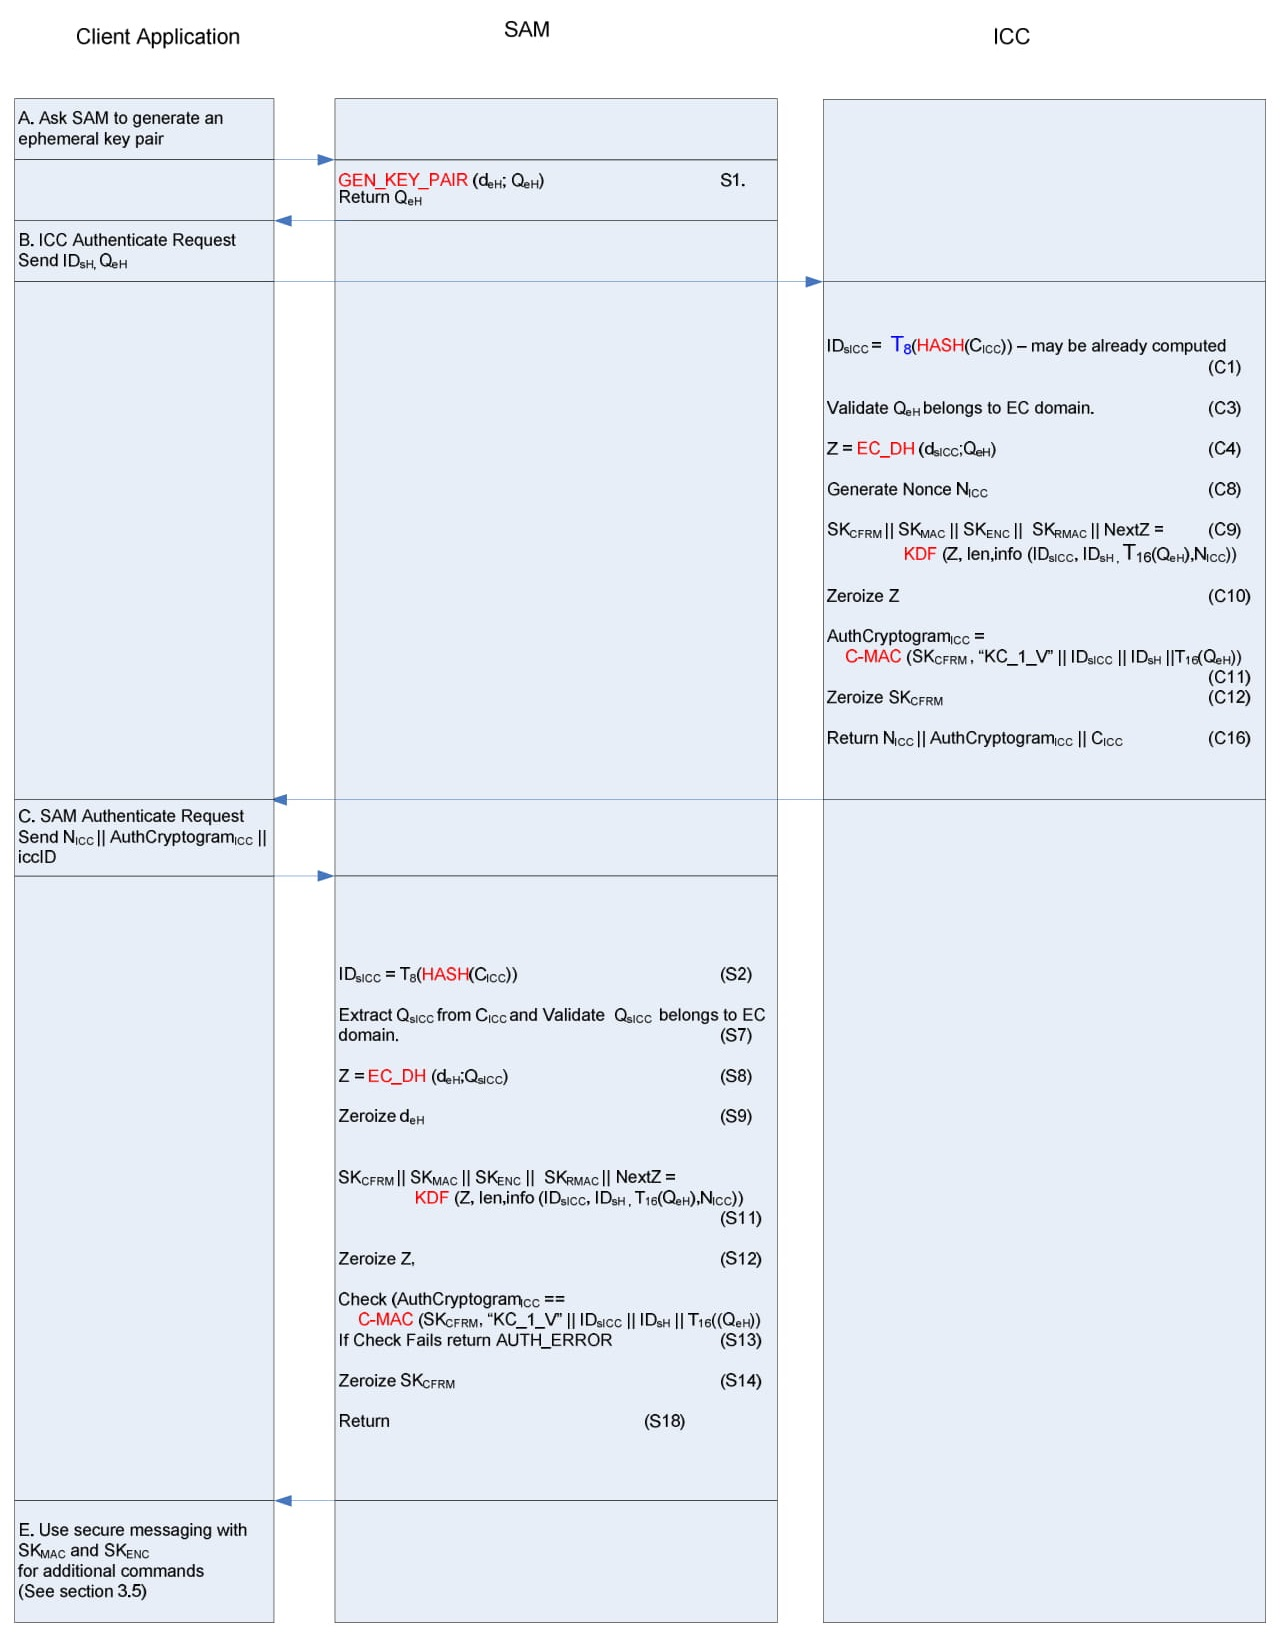
\includegraphics[scale=0.4]{appendix/opacity-zkm}
\subsection{Appendix B - Opacity with Zero Key Management (ZKM-Optimised)}
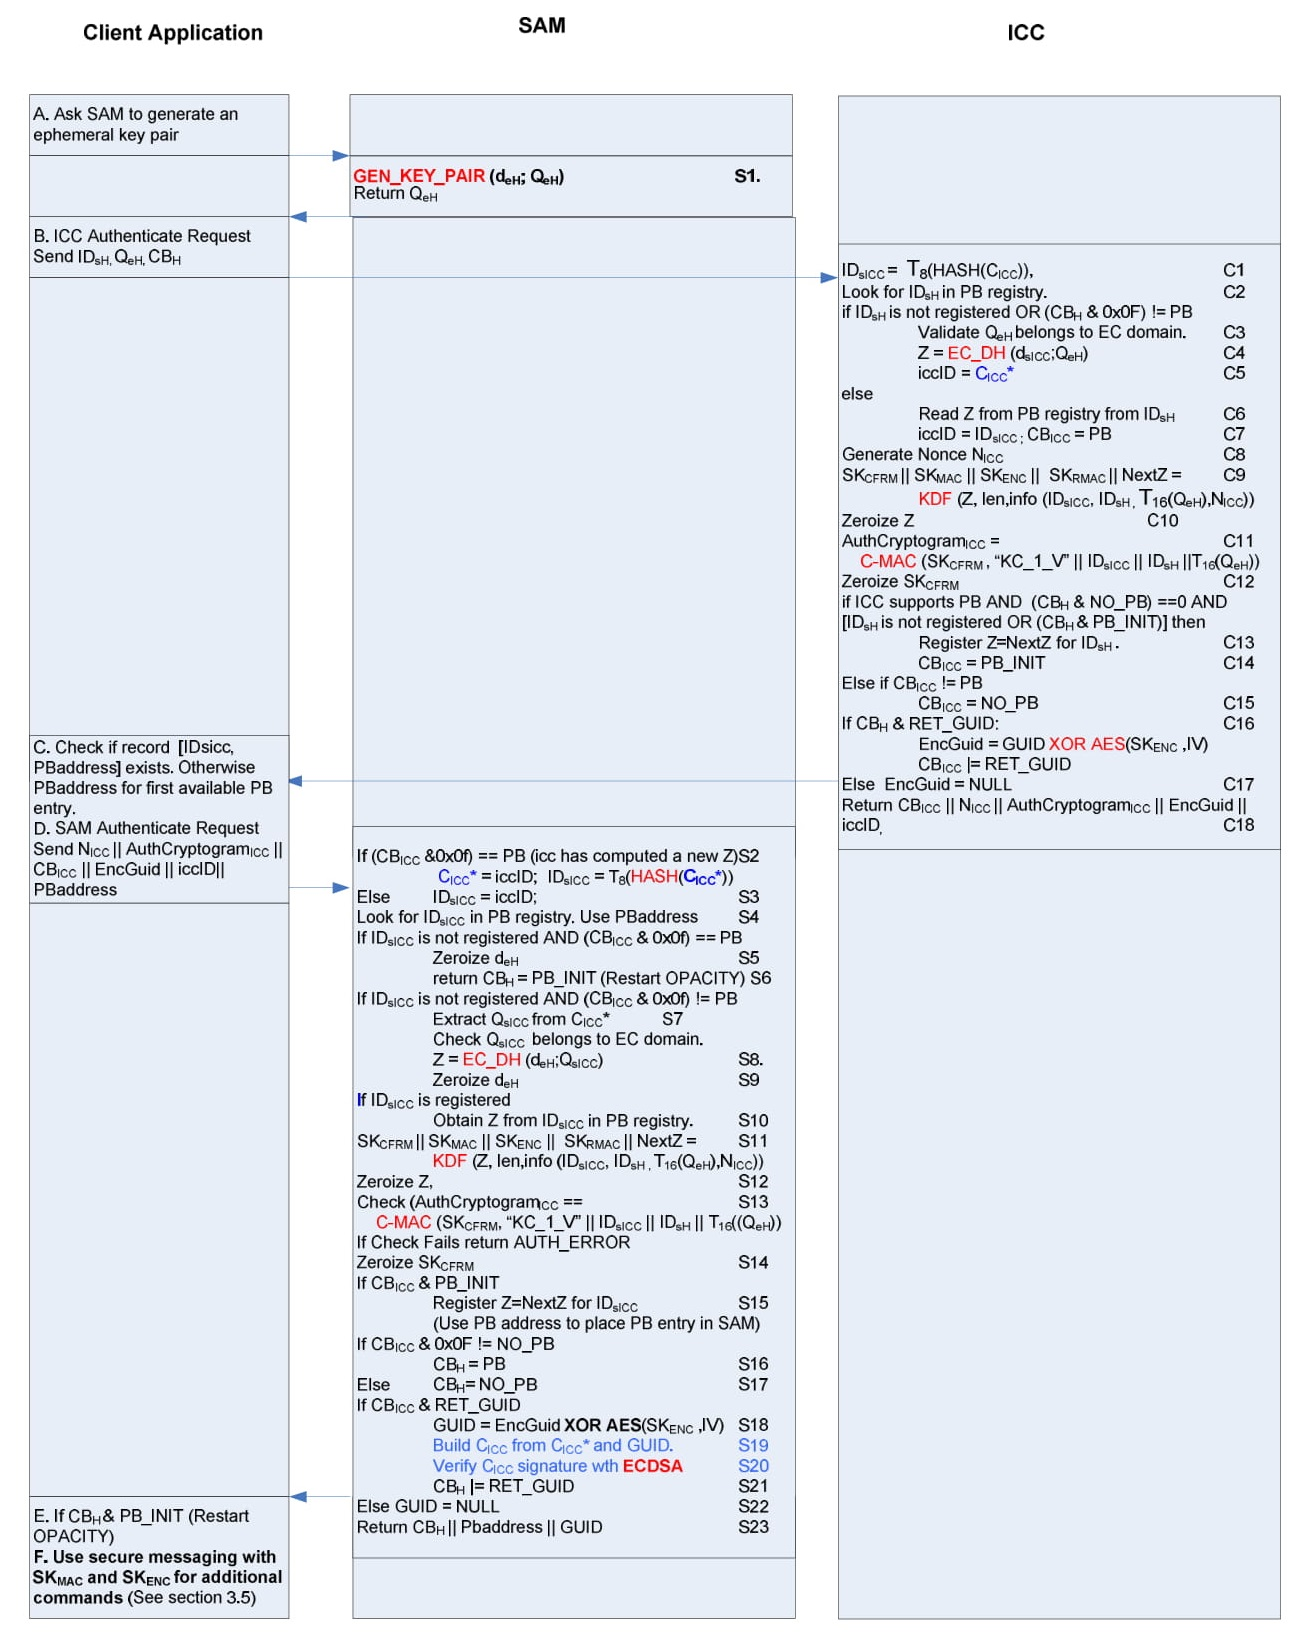
\includegraphics[scale=0.4]{appendix/opacity-zkm-opt}

\subsection{Appendix C - CVC format}
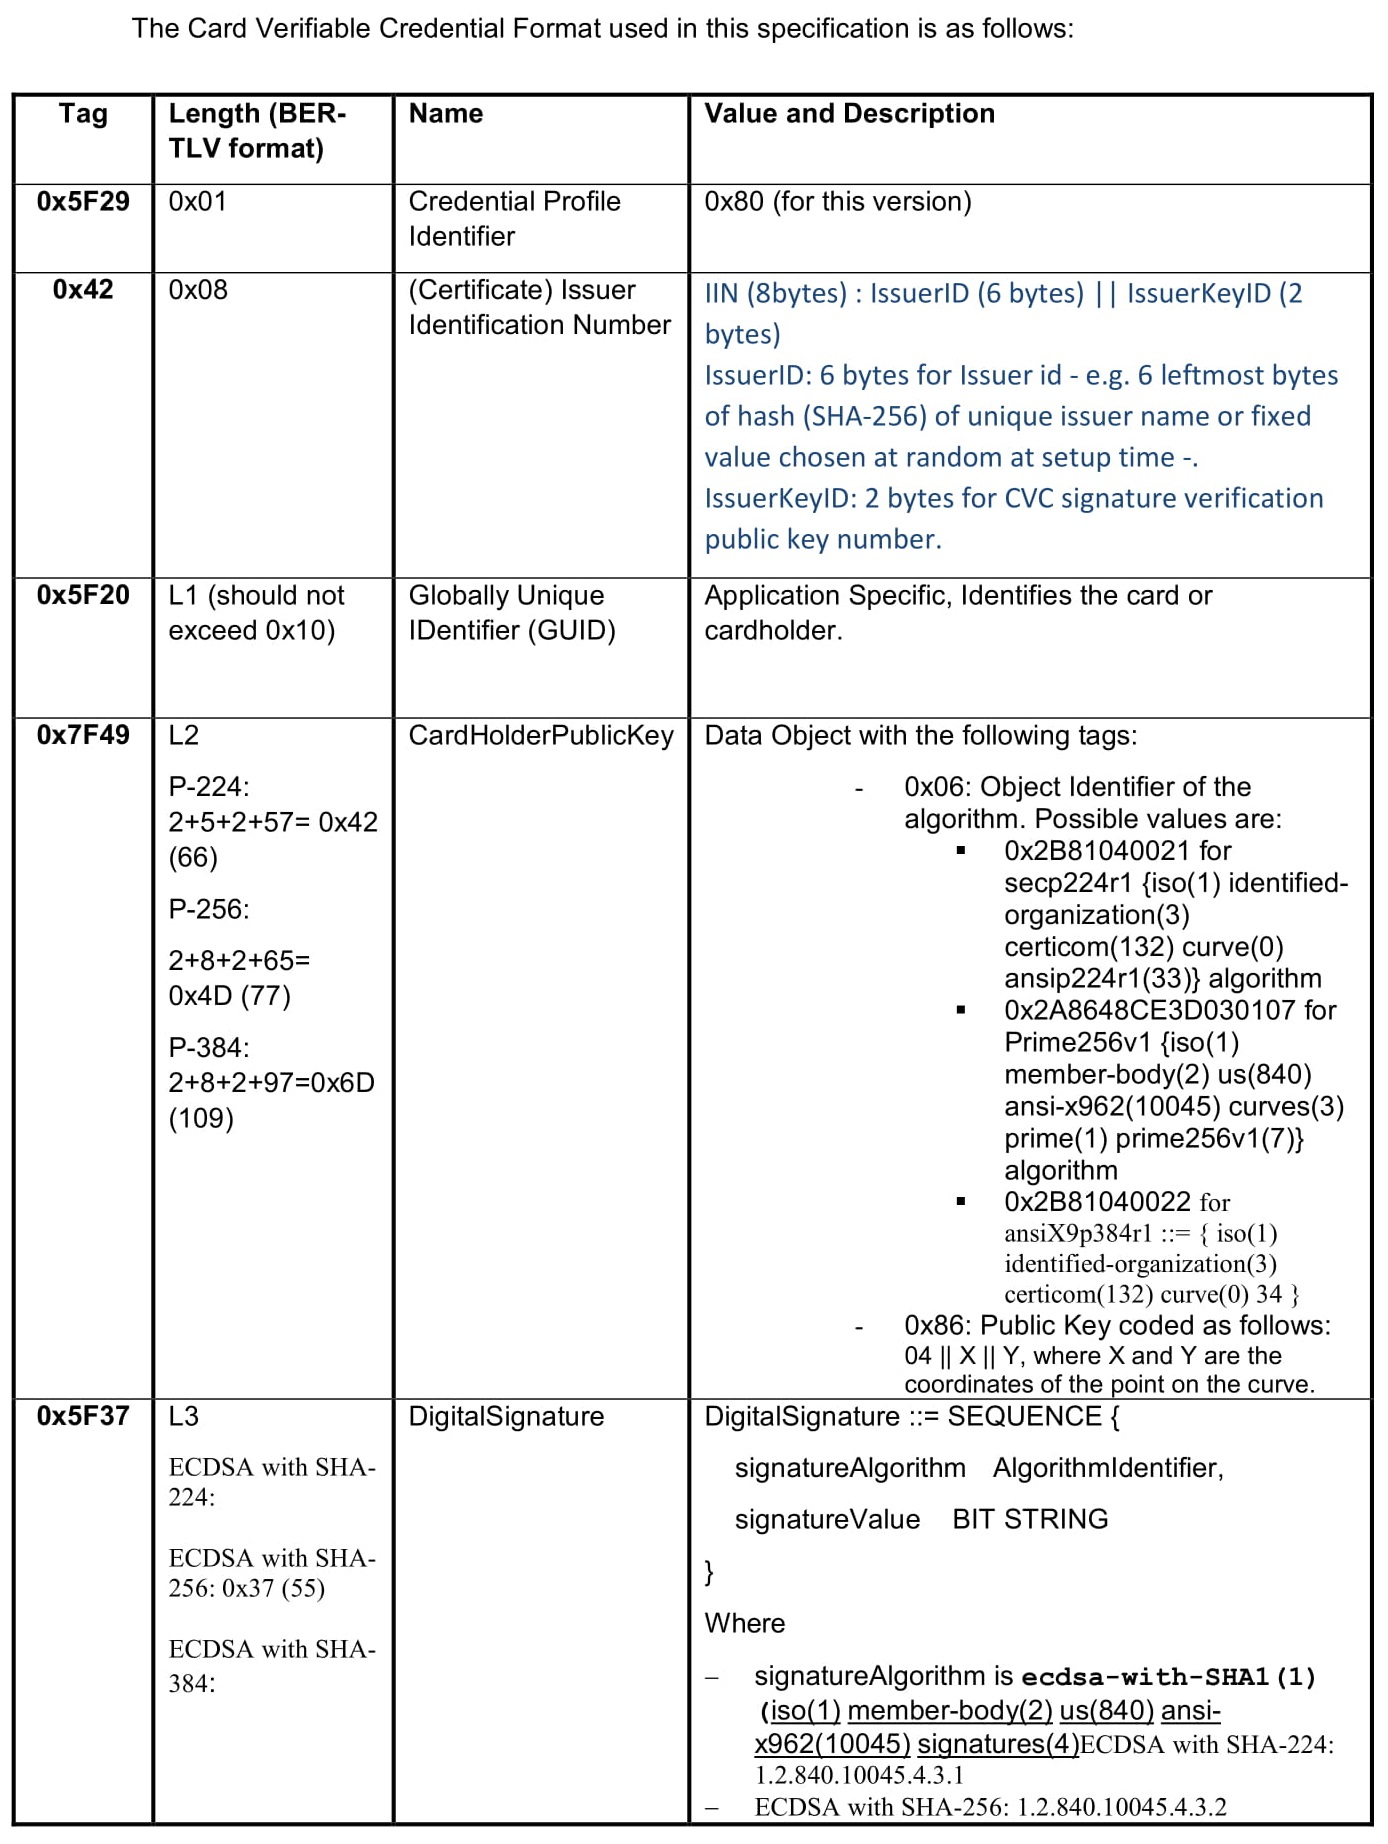
\includegraphics[scale=0.4]{appendix/cvc-1}\\
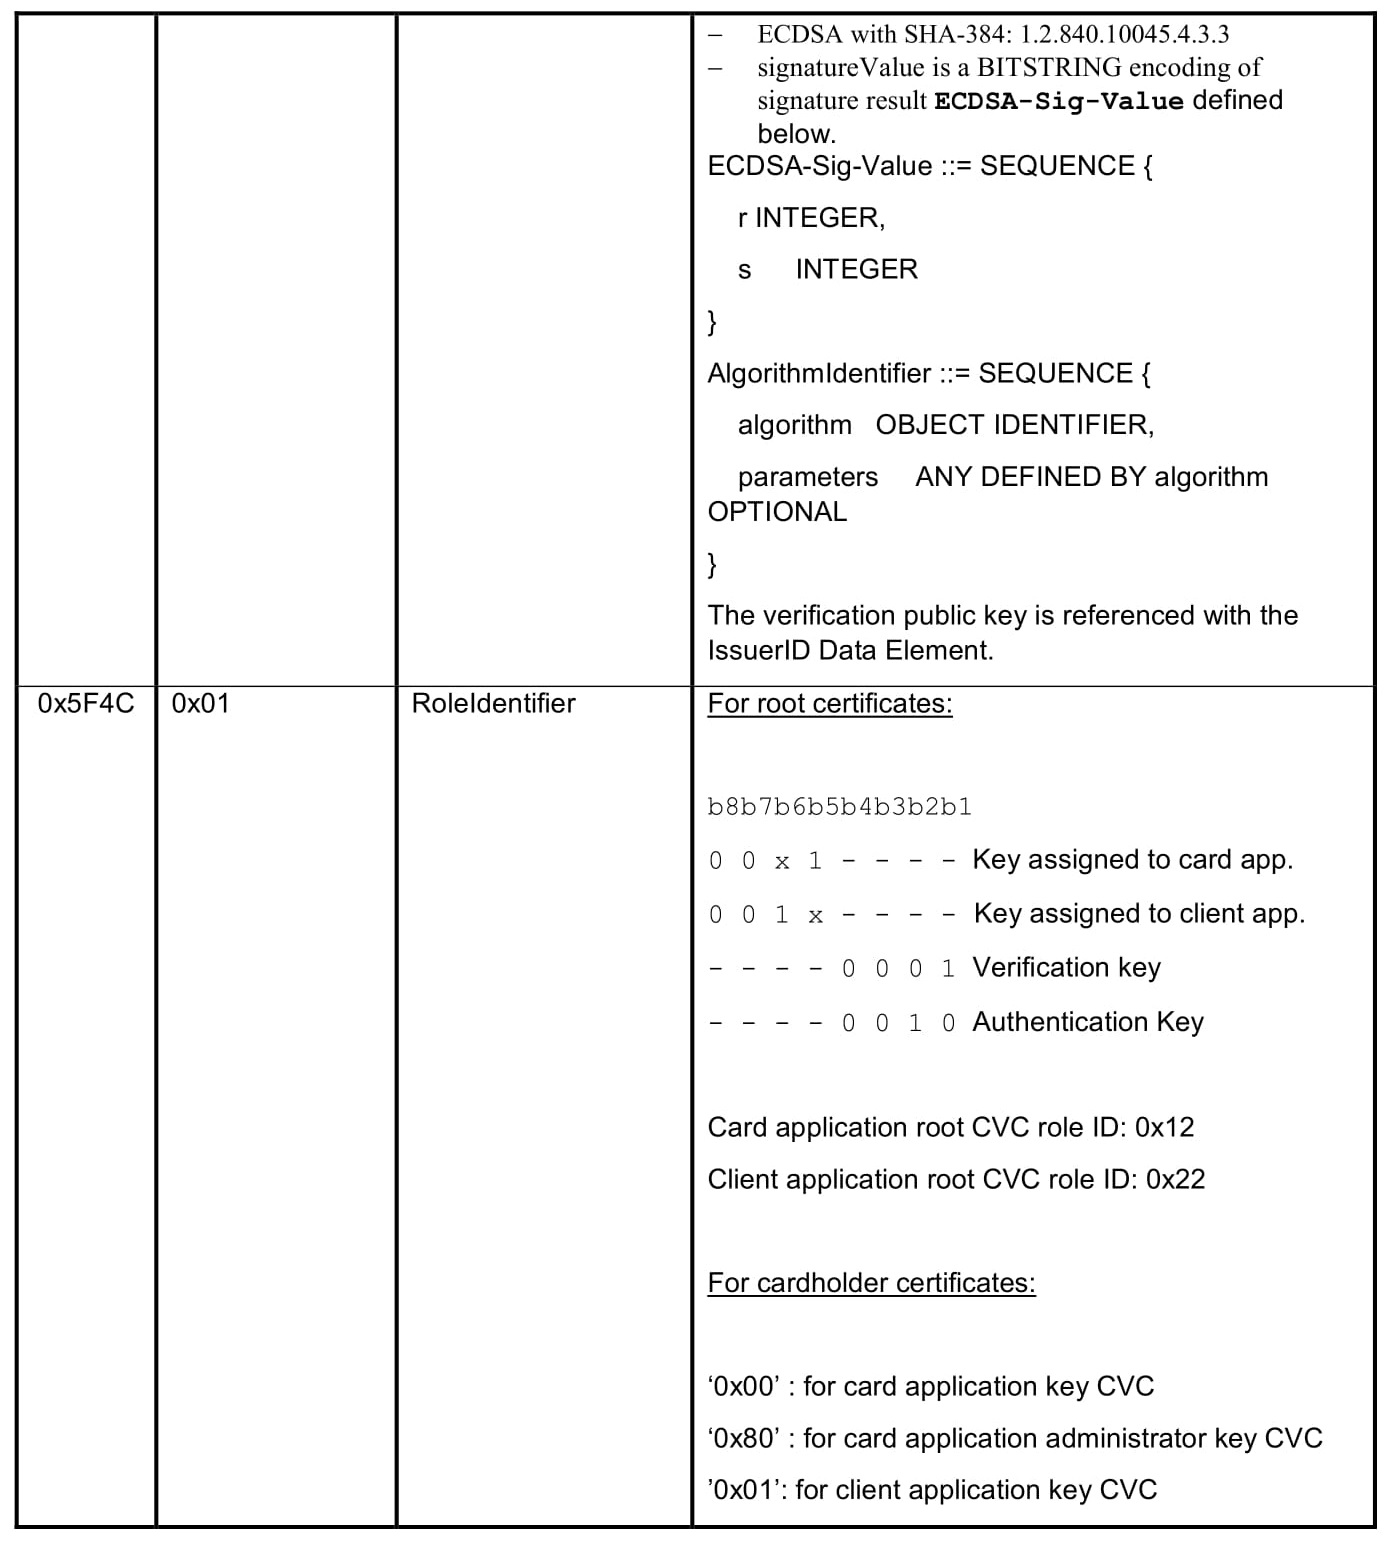
\includegraphics[scale=0.4]{appendix/cvc-2}

Could include C-MAC steps from NIST 800-38B.

\pagebreak

%Index
\section{Index}
TODO (Optional)
\pagebreak

\end{document}
